%\documentclass[handout]{beamer}
\documentclass{beamer}

\mode<presentation>
{
%\usetheme{Singapore}
%\usetheme{Warsaw}
\usetheme{Malmoe}
\useinnertheme{circles}
\useoutertheme{infolines}
% \useinnertheme{rounded}

\setbeamercovered{transparent}
}

\usepackage[english]{babel}
\usepackage[latin1]{inputenc}
\usepackage{bm,textpos,alltt,listings,multirow,ulem}
\usepackage[outputdir=out]{minted}
\usepackage{url}
\usepackage{JedMacros}

% font definitions, try \usepackage{ae} instead of the following
% three lines if you don't like this look
\usepackage{mathptmx}
\usepackage[scaled=.90]{helvet}
\usepackage{courier}
\usepackage[T1]{fontenc}
\usepackage{tikz}
\usetikzlibrary[shapes.arrows,arrows,shapes.misc,chains]


\makeatletter
\def\sectionintoc{}
\def\beamer@sectionintoc#1#2#3#4#5{%
\ifnum\c@tocdepth>0%
\ifnum#4=\beamer@showpartnumber%
{
  \beamer@saveanother%
  \gdef\beamer@todo{}%
  \beamer@slideinframe=#1\relax%
  \expandafter\only\beamer@tocsections{\gdef\beamer@todo{%
      \beamer@tempcount=#5\relax%
      \advance\beamer@tempcount by\beamer@sectionadjust%
      \edef\inserttocsectionnumber{\the\beamer@tempcount}%
      \def\inserttocsection{\hyperlink{Navigation#3}{#2}}%
      \beamer@tocifnothide{\ifnum\c@section=#1\beamer@toc@cs\else\beamer@toc@os\fi}%
      {
        \ifbeamer@pausesections\pause\fi%
        \ifx\beamer@toc@ooss\beamer@hidetext
          \vskip.2em
        \else
          \vskip.2em
        \fi
        {%
          \hbox{\vbox{%
              \def\beamer@breakhere{\\}%
              \beamer@tocact{\ifnum\c@section=#1\beamer@toc@cs\else\beamer@toc@os\fi}    {section in toc}}}%
         \par%
        }%
      }%
    }
  }%
  \beamer@restoreanother%
  }
  \beamer@todo%
  \fi\fi%
}
\makeatother


% \usepackage{pgfpages}
% \pgfpagesuselayout{4 on 1}[letterpaper,landscape,border shrink=5mm]

% Macros for the p-Bratu revision numbers
\def\Rbasic{0}
\def\Rrlap{1}
\def\Rrbratu{2}
\def\Rrpbratu{3}
\def\Rassemblebratu{4}
\def\Rassemblepicard{5}
\def\Rmyprealloc{6}
\def\Rnewtoncrash{7}
\def\Rnewtonbug{8}
\def\Rnewtonfix{9}

\title[https://jedbrown.org/files/201705-MUNPETSc.pdf]{PETSc Tutorial}

\author{Jed Brown\inst{1} \& Kevin Green\inst{2}}


% - Use the \inst command only if there are several affiliations.
% - Keep it simple, no one is interested in your street address.
\institute[CU/ANL,UofS]{\inst{1}CU Boulder and Argonne National Laboratory \and
\inst{2} University of Saskatchewan}

\date{MUN, 2017-05-29/30/31}


% This is only inserted into the PDF information catalog. Can be left
% out.
\subject{Talks}


% If you have a file called "university-logo-filename.xxx", where xxx
% is a graphic format that can be processed by latex or pdflatex,
% resp., then you can add a logo as follows:

% \pgfdeclareimage[height=0.5cm]{university-logo}{university-logo-filename}
% \logo{\pgfuseimage{university-logo}}



% Delete this, if you do not want the table of contents to pop up at
% the beginning of each subsection:
\AtBeginSubsection[]
{
 \begin{frame}<beamer>
 \frametitle{Outline}
 \tableofcontents[currentsection,currentsubsection]
 \end{frame}
}

\AtBeginSection[]{
\begin{frame}<beamer>
  \frametitle{Outline}
  \tableofcontents[currentsection]
\end{frame}
}

% If you wish to uncover everything in a step-wise fashion, uncomment
% the following command:

%\beamerdefaultoverlayspecification{<+->}

\begin{document}
\lstset{language=C}

\begin{frame}
  \titlepage
\end{frame}

\begin{frame}
\frametitle{Outline}
\tableofcontents
% You might wish to add the option [pausesections]
\end{frame}
\input{slides/PETSc/RequestsNotSpecific.tex}


\section{Introduction}
\newcommand\ganttline[4]{% line, tag, start end
   \node at (0,#1*0.4+.1) [anchor=base east] {#2};
   \fill[blue] (#3/\xtick-1991/\xtick,#1*0.4-.1) rectangle (#4/\xtick-1991/\xtick,#1*0.4+.1);}
\newcommand\ganttlabel[6]{% year, label, color, yloc, anchor
  \node[#3] at (#1/\xtick+#6/\xtick-1991/\xtick,#4) [anchor=#5] {#2};
  \fill[#3] (#1/\xtick-1991/\xtick,1/2-.1) rectangle (#1/\xtick-1991/\xtick+0.04,12/2+.6);}

%\begin{frame}{Timeline}
\begin{frame}[shrink=5]{}
\begin{figure}[htbp]
\def\present{2019.2}
\def\xtick{2.4}
\vspace{-1ex}
\begin{tikzpicture}[y=-1cm]
   %\draw[help lines] (0.5,5) grid (8,0.5);
   \ganttlabel{1991}{1991}{red}{7.5}{north}{0}
   \ganttlabel{1995}{1995}{red}{7.5}{north}{0}
   \ganttlabel{2000}{2000}{red}{7.5}{north}{0}
   \ganttlabel{2005}{2005}{red}{7.5}{north}{0}
   \ganttlabel{2010}{2010}{red}{7.5}{north}{0}
   \ganttlabel{2015}{2015}{red}{7.5}{north}{0}
   \ganttlabel{1992}{PETSc-1}{green!70!black}{0}{center}{0}
   \ganttlabel{1994.4}{MPI-1}{magenta!70!black}{-.5}{center}{0}
   \ganttlabel{1997.6}{MPI-2}{magenta!70!black}{-.5}{center}{0}
   \ganttlabel{1995.5}{PETSc-2}{green!70!black}{0}{center}{0}
   \ganttlabel{2008.9}{PETSc-3}{green!70!black}{0}{center}{0}
   \ganttline{1}{Barry}{1991}{\present}
   \ganttline{2}{Bill}{1991}{1996}
   \ganttline{3}{Lois}{1993}{2001}
   \ganttline{4}{Satish}{1997}{\present}
   \ganttline{5}{Dinesh}{1998}{2005.5}
   \ganttline{6}{Hong}{2001}{\present}
   \ganttline{7}{Kris}{2001}{2006}
   \ganttline{8}{Matt}{2001.5}{\present}
   \ganttline{9}{Victor}{2003}{2006.9}
   \ganttline{9}{}{2007.3}{2007.5}
   \ganttline{9}{}{2008.5}{2008.7}
   \ganttline{10}{Dmitry}{2005.6}{2015.6}
   \ganttline{11}{Lisandro}{2006.9}{\present}
   \ganttline{12}{Jed}{2009}{\present}
   \ganttline{13}{Shri}{2009.8}{\present}
   \ganttline{14}{Peter}{2011.6}{2014.5}
   \ganttline{15}{Mark}{2011.9}{\present}
   \ganttline{16}{Stefano}{2012.1}{\present}
   \ganttline{17}{Toby}{2013.3}{\present}
   \ganttline{18}{Mr. Hong}{2014.7}{\present}
\end{tikzpicture}
\end{figure}
\end{frame}

\input{slides/PETSc/About.tex}
\input{slides/PETSc/RoleOfPETSc.tex}
\input{slides/PETSc/BetterthanPETSc.tex}
\input{slides/BillGroppAdvice.tex}
\section{Installation}
\begin{frame}{Downloading}
\begin{itemize}
  \item \url{http://mcs.anl.gov/petsc}, download tarball
  \item We will use Git in this tutorial:
  \begin{itemize}
    \item \url{http://git-scm.com}
    \item Debian/Ubuntu: \shell{aptitude install git}
    \item Fedora: \shell{yum install git}
  \end{itemize}
  \item Get the PETSc maintenance branch
  \begin{itemize}\footnotesize
    \item \shell{\small git clone https://bitbucket.org/petsc/petsc}
    \item \shell{cd petsc}
    \item \shell{git checkout maint}
    \item Get the latest bug fixes with \shell{git pull}
  \end{itemize}
\end{itemize}
\end{frame}

\begin{frame}[fragile]{Configuration}
\begin{block}{Basic configuration}
\begin{itemize}\footnotesize
  \item \shell{export PETSC\_DIR=\$PWD PETSC\_ARCH=intel-dbg}
  \item \shell{./configure -{}-with-mpi-dir=/opt/intel/mpi/impi/intel64/ \mtab \bslash \\
      \qquad\qquad -{}-download-f2cblaslapack \mtab \bslash \\
  	\qquad\qquad -{}-download-\{ml,hypre\}}
  \item \shell{make all test}
\end{itemize}
\end{block}
\begin{itemize}
\item Other common options
  \begin{itemize}\footnotesize
  \item \code{-{}-with-scalar-type=$<$real or complex$>$}
  \item %\code{-{}-with-precision=$<$single,double,__float128$>$}
    \verb|--with-precision=<single,double,__float128>|
  \item \code{-{}-with-64-bit-indices}
  \item \code{-{}-download-\{umfpack,mumps,scalapack,parmetis\}}
  \end{itemize}
\item reconfigure at any time with \\
  {\footnotesize \shell{intel-dbg/conf/reconfigure-intel-dbg.py \mtab\bslash\\
      \qquad\qquad -{}-new-options}}
\end{itemize}
\end{frame}

\frame{
\frametitle{Automatic Downloads}

\begin{itemize}
  \item Most packages can be automatically
  \begin{itemize}
    \item Downloaded
    \item Configured and Built (in {\kb \$PETSC\_DIR/externalpackages})
    \item Installed with PETSc
  \end{itemize}

  \item Currently works for
  \begin{itemize}
    \item petsc4py
    \item PETSc documentation utilities (Sowing, lgrind, c2html)
    \item BLAS, LAPACK, ScaLAPACK, Elemental
    \item MPICH, Open MPI
    \item ParMetis, Chaco, Scotch, Zoltan
    \item MUMPS, SuperLU, SuperLU\_Dist, UMFPack, pARMS, STRUMPACK
    \item PaStiX, FFTW, SPRNG, ViennaCL
    \item HYPRE, ML
    \item Sundials
    \item Triangle, TetGen, FIAT, FFC
    \item HDF5, NetCDF, ExodusII
  \end{itemize}
\end{itemize}
\emph{Can also use \code{-{}-with-xxx-dir=/path/to/your/install}}
}


\begin{frame}{An optimized build}
  \begin{itemize}
  \item \shell{\small intel-dbg/conf/reconfigure-intel-dbg.py \\
      PETSC\_ARCH=intel-opt \\
      -{}-with-debugging=0 \&\& make PETSC\_ARCH=intel-opt}
  \item What does \code{-{}-with-debugging=1} (default) do?
    \begin{itemize}
    \item Keeps debugging symbols (of course)
    \item Maintains a stack so that errors produce a full stack trace (even SEGV)
    \item Does lots of integrity checking of user input
    \item Places sentinels around allocated memory to detect memory errors
    \item Allocates related memory chunks separately (to help find memory bugs)
    \item Keeps track of and reports unused options
    \item Keeps track of and reports allocated memory that is not freed \\
      \quad \code{-malloc\_dump}
    \end{itemize}
  \end{itemize}
\end{frame}


\input{slides/PETSc/Composition.tex}

\section{Objects - Building Blocks of the Code}


\begin{frame}{MPI communicators}
  \begin{itemize}
  \item Opaque object, defines process group and synchronization channel
  \item PETSc objects need an \code{MPI\_Comm} in their constructor
    \begin{itemize}
    \item \code{PETSC\_COMM\_SELF} for serial objects
    \item \code{PETSC\_COMM\_WORLD} common, but \emph{not} required
    \end{itemize}
  \item Can split communicators, spawn processes on new communicators, etc
  \item Operations are one of
    \begin{itemize}
    \item Not Collective: \code{VecGetLocalSize(), MatSetValues()}
    \item Logically Collective: \code{KSPSetType(), PCMGSetCycleType()}
      \begin{itemize}
      \item checked when running in debug mode
      \end{itemize}
    \item Neighbor-wise Collective: \code{VecScatterBegin(), MatMult()}
      \begin{itemize}
      \item Point-to-point communication between two processes
      \item Neighbor collectives in MPI-3
      \end{itemize}
    \item Collective: \code{VecNorm(), MatAssemblyBegin(), KSPCreate()}
      \begin{itemize}
      \item Global communication, synchronous
      \item Non-blocking collectives in MPI-3
      \end{itemize}
    \end{itemize}
  \item Deadlock if some process doesn't participate (\eg wrong order)
  \end{itemize}
\end{frame}




\begin{frame}[fragile]{Objects}
  % \begin{lstlisting}
  %   Mat A;
  %   PetscInt m,n,M,N;
  %   MatCreate(comm,&A);
  %   MatSetSizes(A,m,n,M,N);      /* or PETSC_DECIDE */
  %   MatSetOptionsPrefix(A,"foo_");
  %   MatSetFromOptions(A);
  %   /* Use A */
  %   MatView(A,PETSC_VIEWER_DRAW_WORLD);
  %   MatDestroy(A);
  % \end{lstlisting}
  \begin{minted}{c}
    Mat A;
    PetscInt m,n,M,N;
    MatCreate(comm,&A);
    MatSetSizes(A,m,n,M,N);      /* or PETSC_DECIDE */
    MatSetOptionsPrefix(A,"foo_");
    MatSetFromOptions(A);
    /* Use A */
    MatView(A,PETSC_VIEWER_DRAW_WORLD);
    MatDestroy(A);
  \end{minted}
  \begin{itemize}
  \item \code{Mat} is an opaque object (pointer to incomplete type)
    \oneitem{Assignment, comparison, etc, are cheap}
  \item What's up with this ``Options'' stuff?
    \begin{itemize}
    \item Allows the type to be determined at runtime: \code{-foo\_mat\_type sbaij}
    \item Inversion of Control similar to ``service locator'', \\
      related to ``dependency injection''
    \item Other options (performance and semantics) can be changed at
      runtime under \code{-foo\_mat\_}
    \end{itemize}
  \end{itemize}
\end{frame}

\input{slides/PETSc/PetscObject.tex}

\section{Options Database - Controling the Code}
\begin{frame}{Ways to set options}
  \begin{itemize}
  \item Command line
  \item Filename in the third argument of \code{PetscInitialize()}
  \item \code{$\sim$/.petscrc}
  \item \code{\$PWD/.petscrc}
  \item \code{\$PWD/petscrc}
  \item \code{PetscOptionsInsertFile()}
  \item \code{PetscOptionsInsertString()}
  \item \code{PETSC\_OPTIONS} environment variable
  \item command line option \code{-options\_file [file]}
  \end{itemize}
\end{frame}

\begin{frame}{Try it out}
  \shell{\small cd \$PETSC\_DIR/src/snes/examples/tutorials \&\& make ex5} \\
  \begin{itemize}
  \item \shell{./ex5 -da\_grid\_x 10 -da\_grid\_y 10 -par 6.7 \bslash\\
      -snes\_monitor -\{ksp,snes\}\_converged\_reason \bslash\\
      -snes\_view}
  \item \shell{./ex5 -da\_grid\_x 10 -da\_grid\_y 10 -par 6.7 \bslash\\
      -snes\_monitor -\{ksp,snes\}\_converged\_reason \bslash\\
      -snes\_view -ksp\_view\_mat draw -draw\_pause -1}
  \item \shell{./ex5 -da\_grid\_x 10 -da\_grid\_y 10 -par 6.7 \bslash\\
      -snes\_monitor -\{ksp,snes\}\_converged\_reason \bslash\\
      -snes\_view -pc\_type lu \bslash \\ -pc\_factor\_mat\_ordering\_type natural}
  \item Use \code{-help} to find other ordering types
\end{itemize}
\end{frame}

\begin{frame}[fragile]{Sample output}
\begin{Verbatim}[formatcom=\footnotesize]
  0 SNES Function norm 1.139460779565e+00
  Linear solve converged due to CONVERGED_RTOL iterations 1
  1 SNES Function norm 4.144493702305e-02
  Linear solve converged due to CONVERGED_RTOL iterations 1
  2 SNES Function norm 6.309075568032e-03
  Linear solve converged due to CONVERGED_RTOL iterations 1
  3 SNES Function norm 3.359792279909e-04
  Linear solve converged due to CONVERGED_RTOL iterations 1
  4 SNES Function norm 1.198827244256e-06
  Linear solve converged due to CONVERGED_RTOL iterations 1
  5 SNES Function norm 1.545029314765e-11
\end{Verbatim}
\vspace{-1em}
\includegraphics[width=0.5\textwidth]{figures/Ex5NaturalFill}
\includegraphics[width=0.5\textwidth]{figures/Ex5NDFill}
\end{frame}

\begin{frame}[fragile]{Sample output (SNES and KSP)}
\begin{Verbatim}[formatcom=\footnotesize]
SNES Object: 1 MPI processes
  type: ls
    line search variant: CUBIC
    alpha=1.000000000000e-04, maxstep=1.000000000000e+08, minlambda=1.000000000000e-12
    damping factor=1.000000000000e+00
  maximum iterations=50, maximum function evaluations=10000
  tolerances: relative=1e-08, absolute=1e-50, solution=1e-08
  total number of linear solver iterations=5
  total number of function evaluations=6
  KSP Object:   1 MPI processes
    type: gmres
      GMRES: restart=30, using Classical (unmodified) Gram-Schmidt Orthogonalization with no iterative refinement
      GMRES: happy breakdown tolerance 1e-30
    maximum iterations=10000, initial guess is zero
    tolerances:  relative=1e-05, absolute=1e-50, divergence=10000
    left preconditioning
    using PRECONDITIONED norm type for convergence test
\end{Verbatim}
\end{frame}
\begin{frame}[fragile]{Sample output (PC and Mat)}
\begin{Verbatim}[formatcom=\footnotesize]
  PC Object:   1 MPI processes
    type: lu
      LU: out-of-place factorization
      tolerance for zero pivot 2.22045e-14
      matrix ordering: nd
      factor fill ratio given 5, needed 2.95217
        Factored matrix follows:
          Matrix Object:           1 MPI processes
            type: seqaij
            rows=100, cols=100
            package used to perform factorization: petsc
            total: nonzeros=1358, allocated nonzeros=1358
            total number of mallocs used during MatSetValues calls =0
              not using I-node routines
    linear system matrix = precond matrix:
    Matrix Object:     1 MPI processes
      type: seqaij
      rows=100, cols=100
      total: nonzeros=460, allocated nonzeros=460
      total number of mallocs used during MatSetValues calls =0
        not using I-node routines
\end{Verbatim}
\end{frame}

\begin{frame}{In parallel}
  \begin{itemize}
  \item \shell{mpiexec -n 4 ./ex5 \bslash \\
      \qquad -da\_grid\_x 10 -da\_grid\_y 10 -par 6.7 \bslash\\
      \qquad -snes\_monitor -\{ksp,snes\}\_converged\_reason \bslash\\
      \qquad -snes\_view -sub\_pc\_type lu}
  \item How does the performance change as you
    \begin{itemize}
    \item vary the number of processes (up to 32 or 64)?
    \item increase the problem size?
    \item use an inexact subdomain solve?
    \item try an overlapping method: \code{-pc\_type asm -pc\_asm\_overlap 2}
    \item simulate a big machine: \code{-pc\_asm\_blocks 512}
    \item change the Krylov method: \code{-ksp\_type ibcgs}
    \item use algebraic multigrid: \code{-pc\_type hypre}
    \item use smoothed aggregation multigrid: \code{-pc\_type gamg} or \code{-pc\_type ml}
    \end{itemize}
  \end{itemize}
\end{frame}


\section{Why Parallel?}
\begin{frame}{Why Parallel?}
  \begin{itemize}
  \item Solve a fixed problem faster
  \item Obtain a more accurate solution in the same amount of time
  \item Solve a more complicated problem in the same amount of time
  \item Use more memory than available on one machine
  \end{itemize}
\end{frame}

\begin{frame}{Strong Scaling}
  \begin{center}
    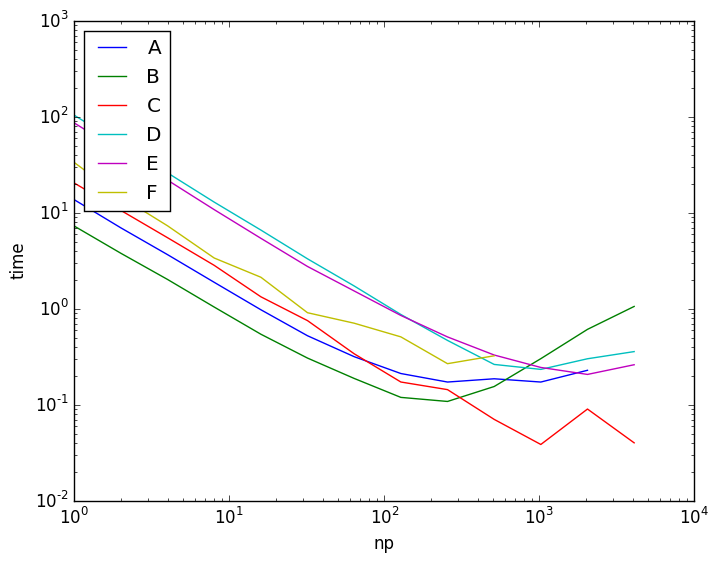
\includegraphics[width=.8\textwidth]{figures/olenz/olenz-time-np}
  \end{center}
  \begin{itemize}
  \item Good: shows absolute time
  \item Bad: log-log plot makes it difficult to discern efficiency
    \begin{itemize}
    \item Stunt 3: \url{http://blogs.fau.de/hager/archives/5835}
    \end{itemize}
  \end{itemize}
\end{frame}

\begin{frame}{Efficiency versus Number of Processes}
  \begin{center}
    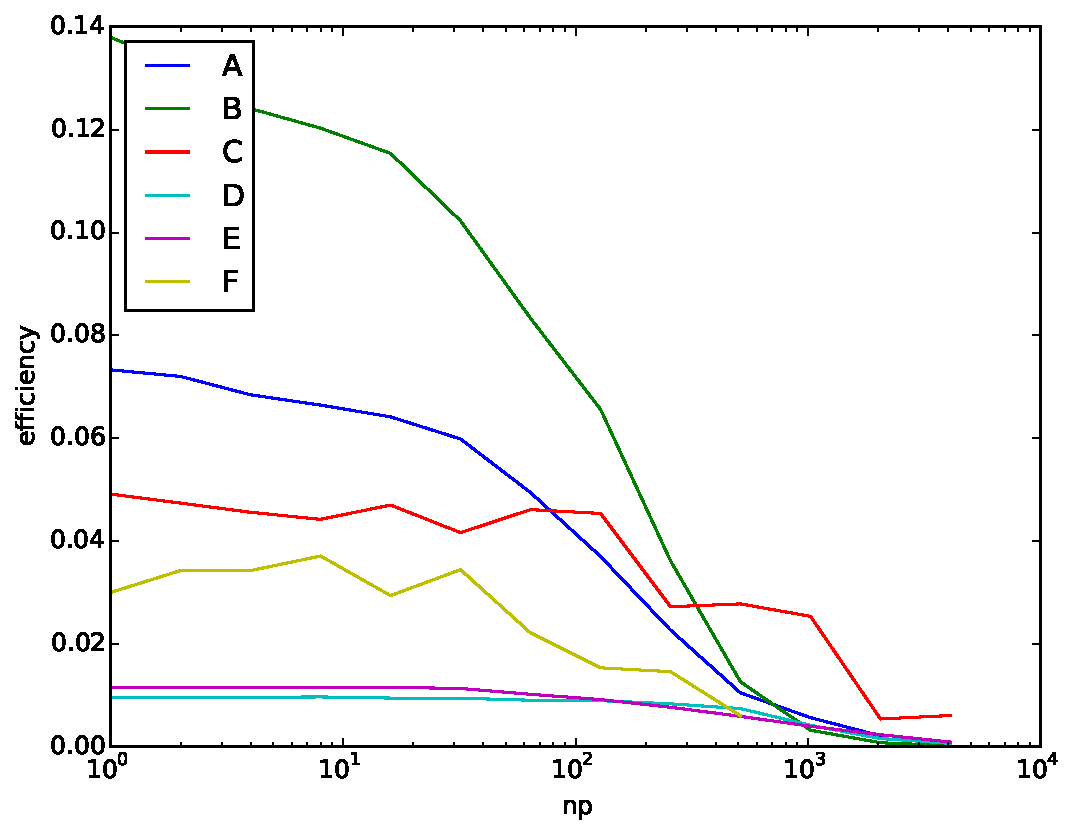
\includegraphics[width=.8\textwidth]{figures/olenz/olenz-efficiency-np}
  \end{center}
  \begin{itemize}
  \item Good: shows efficiency at scale
  \item Bad: no absolute time
  \end{itemize}
\end{frame}

\begin{frame}{Efficiency versus Time}
  \begin{center}
    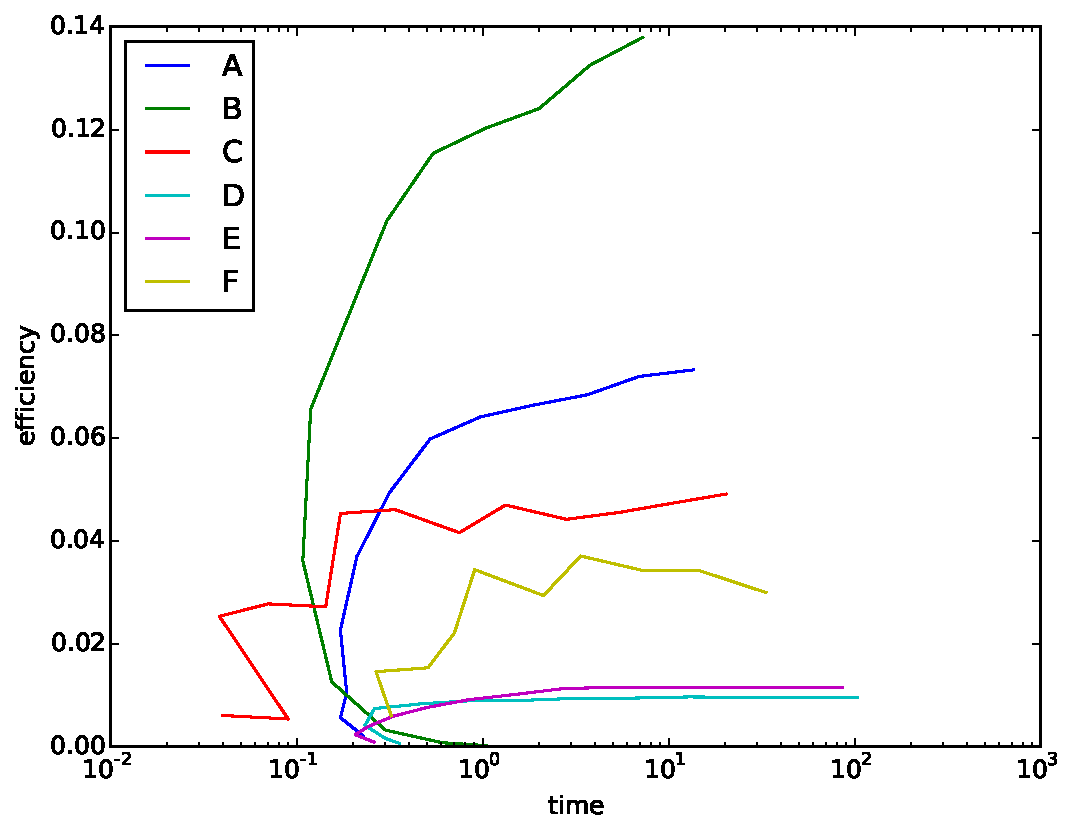
\includegraphics[width=.8\textwidth]{figures/olenz/olenz-efficiency-time}
  \end{center}
  \begin{itemize}
  \item Good: absolute time
  \item Good: efficiency (preferably with units, like DOF/s/process)
  \item Bad: harder to see machine size (but less important)
  \end{itemize}
\end{frame}

\begin{frame}{Scaling Challenges}
  \begin{quote} \centering
    The easiest way to make software scalable \\
    is to make it sequentially inefficient. \\
    (Gropp 1999)
  \end{quote}
  \begin{itemize}
  \item Solver iteration count may increase from
    \begin{itemize}
    \item increased resolution
    \item model parameters (e.g., coefficient contrast/structure)
    \item more realistic models (e.g., plasticity)
    \item model coupling
    \end{itemize}
  \item Algorithm may have suboptimal complexity (e.g., direct solver)
  \item Increasing spatial resolution requires more time steps (usually)
  \item Implementation/data structures may not scale
  \item Architectural effects -- cache, memory
  \end{itemize}
\end{frame}

\begin{frame}{Accuracy-time tradeoffs: \emph{de rigueur} in ODE community}
  \begin{center}
    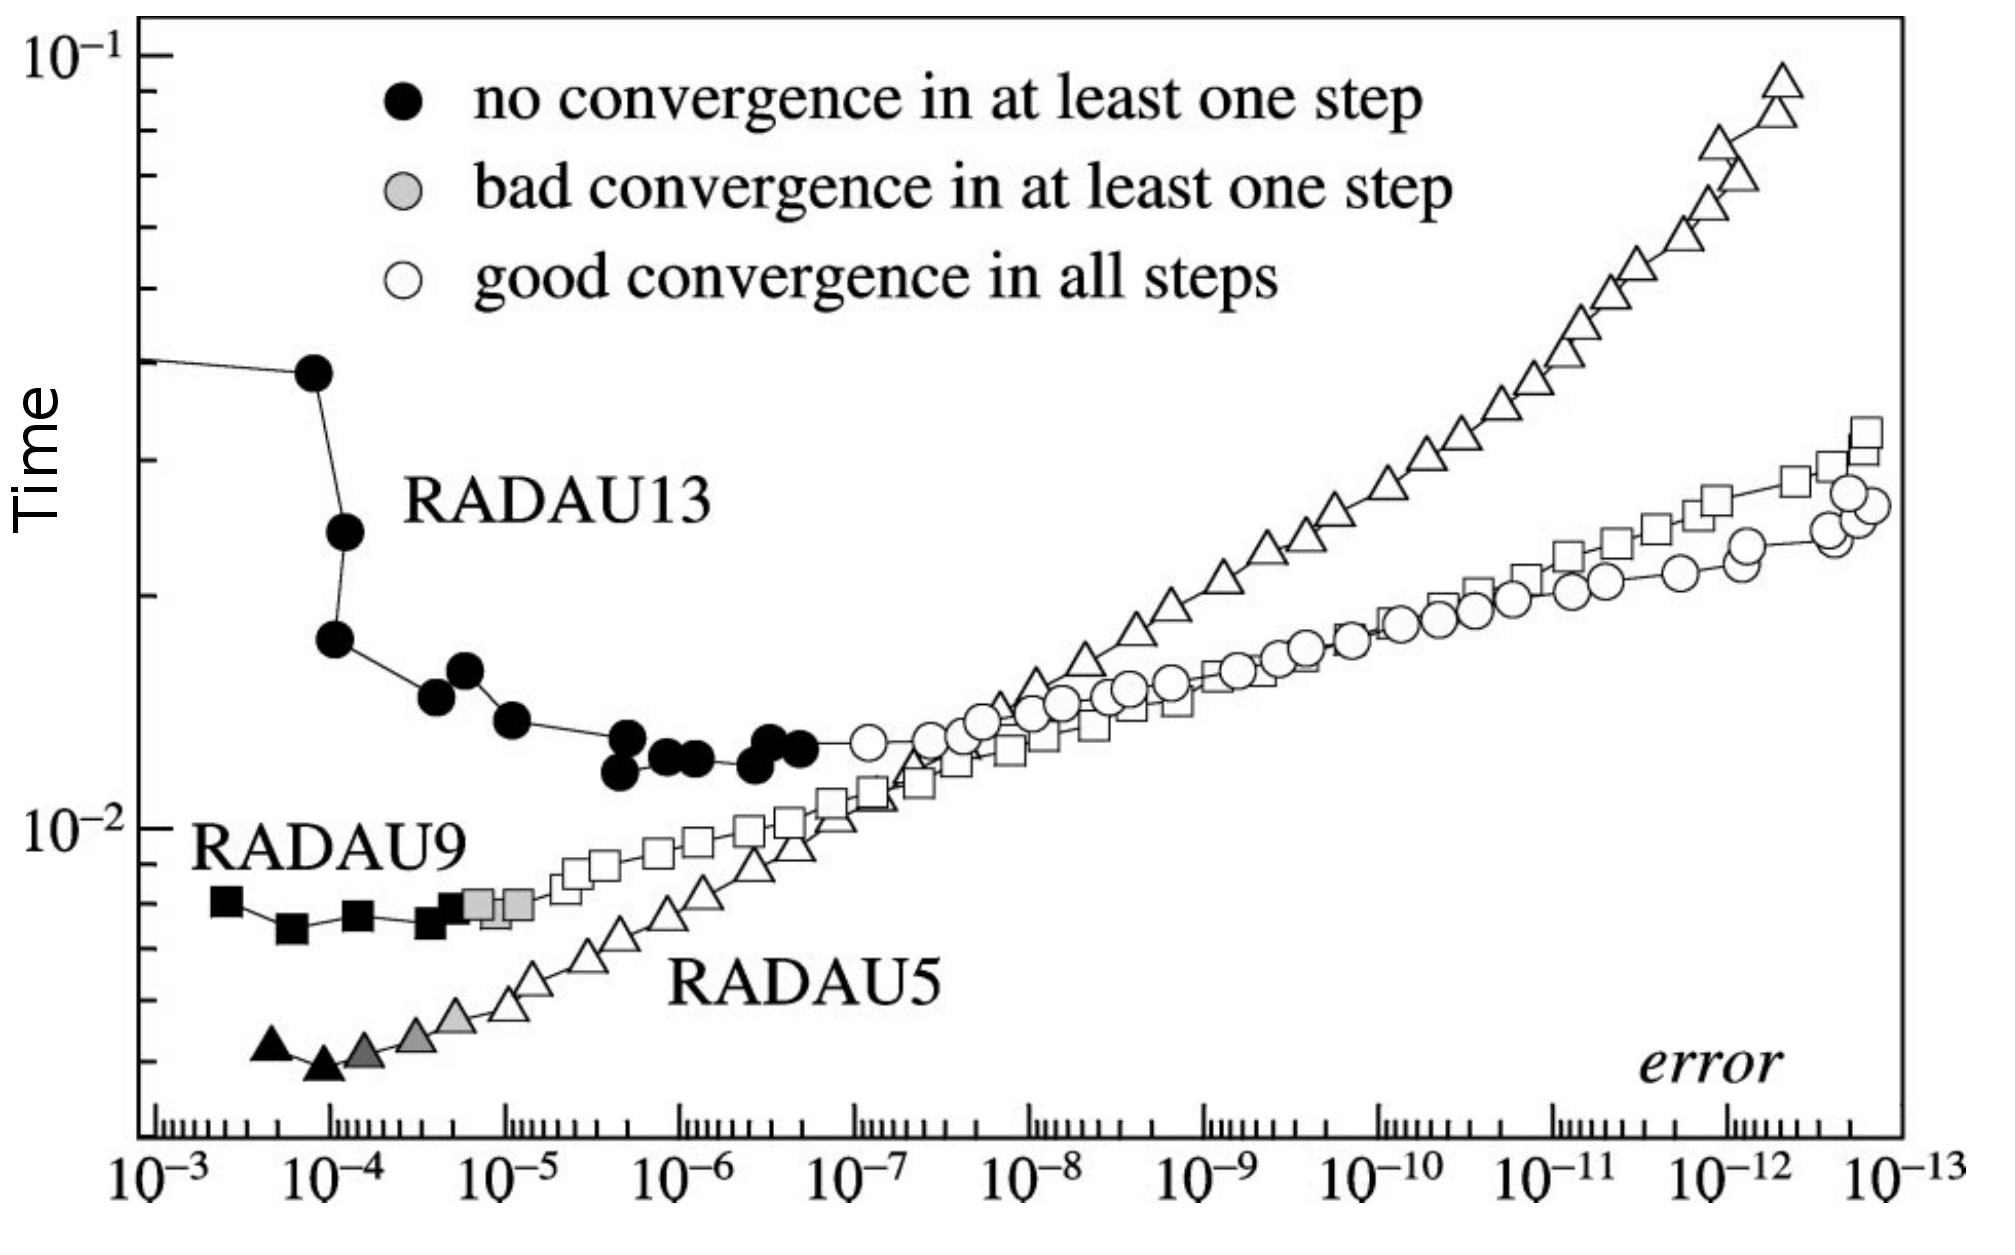
\includegraphics[width=0.8\textwidth]{figures/HairerWanner-WorkPrecision.png}\\
    {\scriptsize [Hairer and Wanner (1999)]}
  \end{center}
  \begin{itemize}
  \item Tests discretization, adaptivity, algebraic solvers, implementation
  \item No reference to number of time steps, number of grid points, etc.
  \end{itemize}
\end{frame}


\section[Core I]{Core PETSc Components and Algorithms Primer}

\subsection{Nonlinear solvers: SNES}
\input{slides/SNES/SNESNewton.tex}
\input{slides/SNES/Callbacks.tex}
\input{slides/SNES/Function.tex}
\begin{frame}[fragile]{SNES Jacobian}
The user provided function that calculates the Jacobian has signature
\begin{minted}{c}
PetscErrorCode (*func)(SNES snes,Vec x,Mat J,
                       Mat Jpre,void *ctx)
\end{minted}

\begin{itemize}
  \item[{\kb x}:] The current solution
  \item[{\kb J}:] The Jacobian
  \item[{\kb Jpre}:] The Jacobian preconditioning matrix (possibly J itself)
  \item[{\kb ctx}:] The user context passed to {\kb SNESSetFunction()}
  \begin{itemize}
    \item Use this to pass application information, e.g. physical constants
  \end{itemize}
\end{itemize}

Alternatively, you can use
\begin{itemize}
  \item a builtin sparse finite difference approximation (``coloring'')
  \item automatic differentiation (ADIC/ADIFOR)
\end{itemize}

\end{frame}


\subsection{Linear Algebra background/theory}
\input{slides/MatrixDefinition.tex}
\input{slides/MatricesImportant.tex}
\input{slides/MatrixNoEntries.tex}
\input{slides/GMRES.tex}
%\subsection{Preconditioning}
\begin{frame}{Preconditioning}
  \begin{block}{Idea: improve the conditioning of the Krylov operator}
    \begin{itemize}
    \item Left preconditioning
      \vspace{-1em}
      \begin{gather*}
        (P^{-1} A) x = P^{-1} b \\
        \{ P^{-1} b, (P^{-1}A) P^{-1} b, (P^{-1}A)^2 P^{-1} b, \dotsc \}
      \end{gather*}
    \item Right preconditioning
      \vspace{-1em}
      \begin{gather*}
        (A P^{-1}) P x = b \\
        \{ b, (A P^{-1}b, (A P^{-1})^2b, \dotsc \}
      \end{gather*}
    \item The product $P^{-1}A$ or $A P^{-1}$ is \emph{not} formed.
    \end{itemize}
  \end{block}
  \begin{definition}[Preconditioner]
      A \emph{preconditioner} $\PP$ is a method for constructing a
matrix (just a linear function, not assembled!)  $P^{-1} = \PP(A,A_p)$
using a matrix $A$ and extra information $A_p$, such that the spectrum
of $P^{-1}A$ (or $A P^{-1}$) is well-behaved.
    \end{definition}
\end{frame}

\input{slides/PreconditionerDefinition.tex}

\begin{frame}{Questions to ask when you see a matrix}
  \begin{enumerate}
  \item What do you want to do with it?
    \begin{itemize}
    \item Multiply with a vector
    \item Solve linear systems or eigen-problems
    \end{itemize}
  \item How is the conditioning/spectrum?
    \begin{itemize}
    \item distinct/clustered eigen/singular values?
    \item symmetric positive definite ($\sigma(A) \subset \R^+$)?
    \item nonsymmetric definite ($\sigma(A) \subset \{z \in \C : \Re [z] > 0 \}$)?
    \item indefinite?
    \end{itemize}
  \item How dense is it?
    \begin{itemize}
    \item block/banded diagonal?
    \item sparse unstructured?
    \item denser than we'd like?
    \end{itemize}
  \item Is there a better way to compute $Ax$?
  \item Is there a different matrix with similar spectrum, but nicer properties?
  \item \alert<2>{How can we precondition $A$?}
  \end{enumerate}
\end{frame}

\begin{frame}{Relaxation}
  Split into lower, diagonal, upper parts: \alert{$ A = L + D + U $}
  \begin{block}{Jacobi \texttt{-pc\_type jacobi}}
    Cheapest preconditioner: $P^{-1} = D^{-1}$
  \end{block}
  \begin{block}{Successive over-relaxation (SOR) \texttt{-pc\_type sor}}
    \begin{gather*}
      \left(L + \frac 1 \omega D\right) x_{n+1} = \left[\left(\frac
          1\omega-1\right)D - U\right] x_n + \omega b \\
      P^{-1} = \text{$k$ iterations starting with $x_0=0$}
    \end{gather*}
    \begin{itemize}
    \item Implemented as a sweep
    \item $\omega = 1$ corresponds to Gauss-Seidel
    \item Very effective at removing high-frequency components of residual
    \end{itemize}
  \end{block}
\end{frame}

\todo{Fundamentals of Richardson convergence}

\begin{frame}[shrink=5]{Factorization}
  Two phases
  \begin{itemize}
  \item symbolic factorization: find where fill occurs, only uses sparsity pattern
  \item numeric factorization: compute factors
  \end{itemize}
  \begin{block}{LU decomposition}
    \begin{itemize}
    \item Ultimate preconditioner
    \item Expensive, for $m\times m$ sparse matrix with bandwidth $b$, traditionally requires $\bigO(mb^2)$ time and $\bigO(mb)$ space.
      \begin{itemize}
      \item Bandwidth scales as $m^{\frac{d-1}{d}}$ in $d$-dimensions
      \item Optimal in 2D: $\bigO(m \cdot \log m)$ space, $\bigO(m^{3/2})$ time
      \item Optimal in 3D: $\bigO(m^{4/3})$ space, $\bigO(m^2)$ time
      \end{itemize}
    \item Symbolic factorization is problematic in parallel
    \end{itemize}
  \end{block}
  \begin{block}{Incomplete LU}
    \begin{itemize}
    \item Allow a limited number of levels of fill:
      ILU($k$)
    \item Only allow fill for entries that exceed threshold: ILUT
    \item Usually poor scaling in parallel
    \item No guarantees
    \item Hierarchical/low-rank representations have potential: STRUMPACK
    \end{itemize}
  \end{block}
\end{frame}

\begin{frame}{1-level Domain decomposition}
  Domain size $L$, subdomain size $H$, element size $h$
  \begin{block}{Overlapping/Schwarz}
    \begin{itemize}\item Solve Dirichlet problems on overlapping
      subdomains
    \item No overlap: $\textit{its} \in \bigO\big( \frac{L}{\sqrt{Hh}} \big)$
    \item Overlap $\delta$: $\textit{its} \in \bigO\big( \frac L {\sqrt{H\delta}} \big)$
    \end{itemize}
  \end{block}
  \vspace{-1ex}
  \begin{block}{Neumann-Neumann}
    \begin{itemize}
    \item Solve Neumann problems on non-overlapping subdomains
    \item $\textit{its} \in \bigO\big( \frac{L}{H}(1+\log\frac H h) \big)$
    \item Tricky null space issues (floating subdomains)
    \item Need subdomain matrices, not globally assembled matrix.
    \end{itemize}
  \end{block}
  \begin{itemize}
  \item Multilevel variants knock off the leading $\frac L H$
  \item Both overlapping and nonoverlapping with this bound
  \end{itemize}
  % \begin{block}{BDDC and FETI-DP}
  %   \begin{itemize}
  %   \item Neumann problems on subdomains with
  %     coarse grid correction
  %   \item $\textit{its} \in \bigO\big(1 + \log\frac H h \big)$
  %   \end{itemize}
  %   \includegraphics[width=0.7\textwidth]{bddc}
  % \end{block}
\end{frame}

\begin{frame}[shrink=5]{Multigrid}
  \begin{block}{Hierarchy: Interpolation and restriction operators}
    \begin{equation*}
    \II^\uparrow : X_{\text{coarse}} \to X_{\text{fine}} \qquad
    \II^\downarrow :  X_{\text{fine}} \to X_{\text{coarse}}
  \end{equation*}
  \end{block}
  \begin{itemize}
  \item Geometric: define problem on multiple levels, use grid to compute hierarchy
  \item Algebraic: define problem only on finest level, use matrix structure to build hierarchy
  \end{itemize}
  \begin{block}{Galerkin approximation}
    Assemble this matrix: $A_{\text{coarse}} = \II^\downarrow A_{\text{fine}} \II^\uparrow$
  \end{block}
  \begin{block}{Application of multigrid preconditioner ($V$-cycle)}
    \begin{itemize}
    \item Apply pre-smoother on fine level (any preconditioner)
    \item Restrict residual to coarse level with $\II^\downarrow$
    \item Solve on coarse level $A_{\text{coarse}} x = r$
    \item Interpolate result back to fine level with $\II^\uparrow$
    \item Apply post-smoother on fine level (any preconditioner)
    \end{itemize}
  \end{block}
\end{frame}

\begin{frame}{Multigrid convergence properties}
  \begin{itemize}
  \item Textbook: $P^{-1}A$ is spectrally equivalent to identity
    \begin{itemize}
    \item Constant number of iterations to converge up to discretization error
    \end{itemize}
  \item Most theory applies to SPD systems
    \begin{itemize}
    \item variable coefficients (\eg discontinuous): low energy interpolants
    \item mesh- and/or physics-induced anisotropy: semi-coarsening/line smoothers
    \item complex geometry: difficult to have meaningful coarse levels
    \end{itemize}
  \item Deeper algorithmic difficulties
    \begin{itemize}
    \item nonsymmetric (\eg advection, shallow water, Euler) \\
    \item indefinite (\eg incompressible flow, Helmholtz)
    \end{itemize}
  \item Performance considerations
    \begin{itemize}
    \item Aggressive coarsening is critical in parallel
    \item Most theory uses SOR smoothers, ILU often more robust
    \item Coarsest level usually solved semi-redundantly with direct solver
    \end{itemize}
  \item Multilevel Schwarz is essentially the same with different language
    \begin{itemize}
    \item assume strong smoothers, emphasize aggressive coarsening
    \end{itemize}
  \end{itemize}
\end{frame}

\begin{frame}{Norms}
  \begin{itemize}
  \item Krylov subspace: $\{P^{-1}b,(P^{-1}A)P^{-1}b,(P^{-1}A)^2P^{-1}b,\dotsc\}$
  \item Subspace needs to contain the solution
    \begin{itemize}
    \item Diameter of preconditioned connectivity graph
    \end{itemize}
  \item Need to find the correct linear combination
    \begin{itemize}
    \item Optimize unpreconditioned residual norm (usually right preconditioning)
      \begin{equation*}
        \norm{A x - b}_2 = \norm{A (x - x^*)}_2 = \norm{x-x^*}_{A^T A}
      \end{equation*}
    \item Optimize preconditioned residual norm (usually left preconditioning)
      \begin{equation*}
        \norm{P^{-1} (A x - b)}_2 = \norm{P^{-1}A (x - x^*)}_2 = \norm{x-x^*}_{A^T P^{-T} P^{-1} A}
      \end{equation*}
    \item Natural norm (conjugate gradients) minimizes $\norm{x-x^*}_{P^{-1/2}AP^{-1/2}}$
    \end{itemize}
  \item Evaluating convergence
    \begin{itemize}
    \item Preconditioned, unpreconditioned, or natural norm
    \item Which one to trust?
    \item \code{-ksp\_monitor\_true\_residual}, \code{-ksp\_norm\_type}
    \end{itemize}
  \end{itemize}
\end{frame}


\subsection{Structured grid distribution: DMDA}
\input{slides/DM/DMDA.tex}
\input{slides/DA/GhostValues.tex}
\input{slides/DA/GlobalNumberings.tex}
\input{slides/DA/LocalNumbering.tex}
\input{slides/DA/Vectors.tex}
\input{slides/DA/UpdatingGhosts.tex}
\input{slides/DA/Stencils.tex}
\input{slides/DA/CreatingDA2d.tex}
\input{slides/DA/WorkingWithLocal.tex}
\frame{
\frametitle{DA Local Function}

The user provided function which calculates the nonlinear residual in 2D has signature \\
{\kb PetscErrorCode (*lfunc)(DMDALocalInfo *info, \\
  \qquad \qquad \qquad Field **x, Field **r, void *ctx)}
\begin{columns}\begin{column}{0.15\textwidth}\end{column}\begin{column}{0.85\textwidth}
\begin{itemize}
  \item[{\kb info}:] All layout and numbering information
  \item[{\kb x}:] The current solution
  \begin{itemize}
    \item Notice that it is a multidimensional array
  \end{itemize}
  \item[ {\kb r}:] The residual
  \item[ {\kb ctx}:] The user context passed to {\kb DMSetApplicationContext()} or to SNES
\end{itemize}
\end{column}\end{columns}

\bigskip

The local DMDA function is activated by calling
\begin{itemize}
\item {\kb SNESSetDM(snes,dm);}
\item {\kb DMDASNESSetFunctionLocal(dm, InsertMode imode, lfunc, ctx);} \\
  where {\kb imode} is {\kb INSERT\_VALUES} or {\kb ADD\_VALUES}
\end{itemize}
}

\input{slides/DA/BratuResidual.tex}

\begin{frame}{Other DMs}
  \begin{itemize}
  \item DMPlex - sophisticated dimension-independent management of unstructured meshes as a CW complex
  \item DMForest - interface to p4est, a highly scalable adaptive forest of quadtree/octree library
  \item DMNetwork - for discrete networks like power grids and circuits
  \end{itemize}
\end{frame}


\subsection{Profiling}
\begin{frame}{Profiling}

\begin{itemize}
  \item Use {\kb -log\_view} for a performance profile
  \begin{itemize}
    \item Event timing
    \item Event flops
    \item Memory usage
    \item MPI messages
  \end{itemize}

  \item Call {\kb PetscLogStagePush()} and {\kb PetscLogStagePop()}
  \begin{itemize}
    \item User can add new stages
  \end{itemize}

  \item Call {\kb PetscLogEventBegin()} and {\kb PetscLogEventEnd()}
  \begin{itemize}
    \item User can add new events
  \end{itemize}

  \item Call {\kb PetscLogFlops()} to include your flops
\end{itemize}

\end{frame}

\begin{frame}[fragile]{Reading \code{-log\_view}}
\begin{itemize}
\item
{\scriptsize
\begin{verbatim}
                         Max       Max/Min        Avg      Total 
Time (sec):           1.548e+02      1.00122   1.547e+02
Objects:              1.028e+03      1.00000   1.028e+03
Flops:                1.519e+10      1.01953   1.505e+10  1.204e+11
Flops/sec:            9.814e+07      1.01829   9.727e+07  7.782e+08
MPI Messages:         8.854e+03      1.00556   8.819e+03  7.055e+04
MPI Message Lengths:  1.936e+08      1.00950   2.185e+04  1.541e+09
MPI Reductions:       2.799e+03      1.00000
\end{verbatim}}
\item Also a summary per stage
\item Memory usage per stage (based on when it was allocated)
\item Time, messages, reductions, balance, flops per event per stage
\item Always send \code{-log\_view} when asking performance questions on
  mailing list
\end{itemize}
\end{frame}

\begin{frame}[fragile]{Reading \code{-log\_view}}
\begin{Verbatim}[formatcom=\tiny]
Event                Count      Time (sec)     Flops                             --- Global ---  --- Stage ---   Total
                   Max Ratio  Max     Ratio   Max  Ratio  Mess   Avg len Reduct  %T %F %M %L %R  %T %F %M %L %R Mflop/s
------------------------------------------------------------------------------------------------------------------------
--- Event Stage 1: Full solve
VecDot                43 1.0 4.8879e-02 8.3 1.77e+06 1.0 0.0e+00 0.0e+00 4.3e+01  0  0  0  0  0   0  0  0  0  1 73954
VecMDot             1747 1.0 1.3021e+00 4.6 8.16e+07 1.0 0.0e+00 0.0e+00 1.7e+03  0  1  0  0 14   1  1  0  0 27 128346
VecNorm             3972 1.0 1.5460e+00 2.5 8.48e+07 1.0 0.0e+00 0.0e+00 4.0e+03  0  1  0  0 31   1  1  0  0 61 112366
VecScale            3261 1.0 1.6703e-01 1.0 3.38e+07 1.0 0.0e+00 0.0e+00 0.0e+00  0  0  0  0  0   0  0  0  0  0 414021
VecScatterBegin     4503 1.0 4.0440e-01 1.0 0.00e+00 0.0 6.1e+07 2.0e+03 0.0e+00  0  0 50 26  0   0  0 96 53  0     0
VecScatterEnd       4503 1.0 2.8207e+00 6.4 0.00e+00 0.0 0.0e+00 0.0e+00 0.0e+00  0  0  0  0  0   0  0  0  0  0     0
MatMult             3001 1.0 3.2634e+01 1.1 3.68e+09 1.1 4.9e+07 2.3e+03 0.0e+00 11 22 40 24  0  22 44 78 49  0 220314
MatMultAdd           604 1.0 6.0195e-01 1.0 5.66e+07 1.0 3.7e+06 1.3e+02 0.0e+00  0  0  3  0  0   0  1  6  0  0 192658
MatMultTranspose     676 1.0 1.3220e+00 1.6 6.50e+07 1.0 4.2e+06 1.4e+02 0.0e+00  0  0  3  0  0   1  1  7  0  0 100638
MatSolve            3020 1.0 2.5957e+01 1.0 3.25e+09 1.0 0.0e+00 0.0e+00 0.0e+00  9 21  0  0  0  18 41  0  0  0 256792
MatCholFctrSym         3 1.0 2.8324e-04 1.0 0.00e+00 0.0 0.0e+00 0.0e+00 0.0e+00  0  0  0  0  0   0  0  0  0  0     0
MatCholFctrNum        69 1.0 5.7241e+00 1.0 6.75e+08 1.0 0.0e+00 0.0e+00 0.0e+00  2  4  0  0  0   4  9  0  0  0 241671
MatAssemblyBegin     119 1.0 2.8250e+00 1.5 0.00e+00 0.0 2.1e+06 5.4e+04 3.1e+02  1  0  2 24  2   2  0  3 47  5     0
MatAssemblyEnd       119 1.0 1.9689e+00 1.4 0.00e+00 0.0 2.8e+05 1.3e+03 6.8e+01  1  0  0  0  1   1  0  0  0  1     0
SNESSolve              4 1.0 1.4302e+02 1.0 8.11e+09 1.0 6.3e+07 3.8e+03 6.3e+03 51 50 52 50 50  99100 99100 97 113626
SNESLineSearch        43 1.0 1.5116e+01 1.0 1.05e+08 1.1 2.4e+06 3.6e+03 1.8e+02  5  1  2  2  1  10  1  4  4  3 13592
SNESFunctionEval      55 1.0 1.4930e+01 1.0 0.00e+00 0.0 1.8e+06 3.3e+03 8.0e+00  5  0  1  1  0  10  0  3  3  0     0
SNESJacobianEval      43 1.0 3.7077e+01 1.0 7.77e+06 1.0 4.3e+06 2.6e+04 3.0e+02 13  0  4 24  2  26  0  7 48  5   429
KSPGMRESOrthog      1747 1.0 1.5737e+00 2.9 1.63e+08 1.0 0.0e+00 0.0e+00 1.7e+03  1  1  0  0 14   1  2  0  0 27 212399
KSPSetup             224 1.0 2.1040e-02 1.0 0.00e+00 0.0 0.0e+00 0.0e+00 3.0e+01  0  0  0  0  0   0  0  0  0  0     0
KSPSolve              43 1.0 8.9988e+01 1.0 7.99e+09 1.0 5.6e+07 2.0e+03 5.8e+03 32 49 46 24 46  62 99 88 48 88 178078
PCSetUp              112 1.0 1.7354e+01 1.0 6.75e+08 1.0 0.0e+00 0.0e+00 8.7e+01  6  4  0  0  1  12  9  0  0  1 79715
PCSetUpOnBlocks     1208 1.0 5.8182e+00 1.0 6.75e+08 1.0 0.0e+00 0.0e+00 8.7e+01  2  4  0  0  1   4  9  0  0  1 237761
PCApply              276 1.0 7.1497e+01 1.0 7.14e+09 1.0 5.2e+07 1.8e+03 5.1e+03 25 44 42 20 41  49 88 81 39 79 200691
\end{Verbatim}
\end{frame}

\begin{frame}{Communication Costs}
  \begin{itemize}
  \item Reductions: usually part of Krylov method, latency limited
    \begin{itemize}
    \item \code{VecDot}
    \item \code{VecMDot}
    \item \code{VecNorm}
    \item \code{MatAssemblyBegin}
    \item Change algorithm (e.g. IBCGS, PGMRES)
    \end{itemize}
  \item Point-to-point (nearest neighbor), latency or bandwidth
    \begin{itemize}
    \item \code{VecScatter}
    \item \code{MatMult}
    \item \code{PCApply}
    \item \code{MatAssembly}
    \item \code{SNESFunctionEval}
    \item \code{SNESJacobianEval}
    \item Compute subdomain boundary fluxes redundantly
    \item Ghost exchange for all fields at once, or overlap
    \item Better partition
    \end{itemize}
  \end{itemize}
\end{frame}

\begin{frame}{HPGMG-FE \quad \url{https://hpgmg.org}}
  \centering 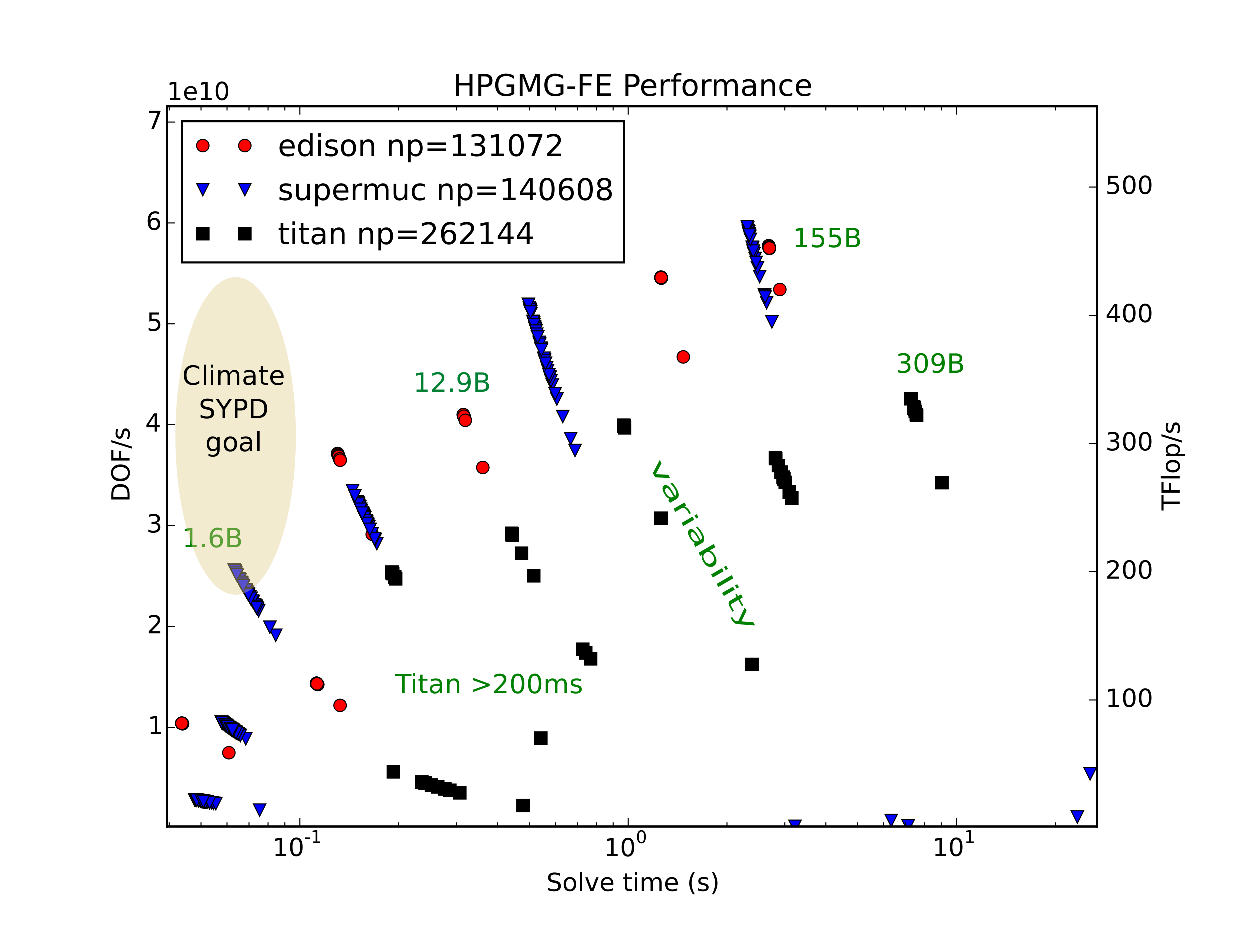
\includegraphics[width=.9\textwidth]{figures/hpgmg/range-edison-supermuc-titan-ann2}
\end{frame}


\subsection{Matrix Redux}
\begin{frame}{Matrices, redux}
What are PETSc matrices?
\begin{itemize}
\item Linear operators on finite dimensional vector spaces. (snarky)
  \item<2> Fundamental objects for storing stiffness matrices and Jacobians
  \item<2> Each process locally owns a contiguous set of rows
  \item<2> Supports many data types
  \begin{itemize}
    \item AIJ, Block AIJ, Symmetric AIJ, Block Diagonal, etc.
  \end{itemize}
  \item<2> Supports structures for many packages
  \begin{itemize}
    \item MUMPS, SuperLU, UMFPack, Hypre, Elemental
  \end{itemize}
\end{itemize}
\end{frame}

\begin{frame}{How do I create matrices?}

\begin{itemize}
  \item {\kb MatCreate(MPI\_Comm, Mat *)}
  \item {\kb MatSetSizes(Mat, int m, int n, int M, int N)}
  \item {\kb MatSetType(Mat, MatType typeName)}
  \item {\kb MatSetFromOptions(Mat)}
  \begin{itemize}
    \item Can set the type at runtime
  \end{itemize}
  \item {\kb MatSetBlockSize(Mat, int bs)}
    \oneitem{for vector problems}
  \item {\kb MatXAIJSetPreallocation(Mat,...)} %(Mat,int bs,int d_nz,const int
                                %d_nnz[],int o_nz,const int o_nnz[])}
    \oneitem{important for assembly performance}
  \item {\kb MatSetValues(Mat,...)}
  \begin{itemize}
    \item {\bf MUST} be used, but does automatic communication
    \item \cfunc|MatSetValuesLocal|, \cfunc|MatSetValuesStencil|
    \item \cfunc|MatSetValuesBlocked|
  \end{itemize}
\end{itemize}
\end{frame}

\input{slides/PETSc/Integration/MatrixPolymorphism.tex}
\input{slides/PETSc/Integration/MatrixAssembly.tex}
\begin{frame}[fragile]{A Scalable Way to Set the Elements of a Matrix}{Simple 3-point stencil for 1D Laplacian}
\small
\begin{minted}{c}
v[0] = -1.0; v[1] = 2.0; v[2] = -1.0;
for (row = start;  row < end; row++) {
  cols[0] = row-1; cols[1] = row; cols[2] = row+1;
  if (row == 0) {
    MatSetValues(A,1,&row,2,&cols[1],&v[1],INSERT_VALUES);
  } else if (row == N-1) {
    MatSetValues(A,1,&row,2,cols,v,INSERT_VALUES);
  } else {
    MatSetValues(A,1,&row,3,cols,v,INSERT_VALUES);
  }
}
MatAssemblyBegin(A, MAT_FINAL_ASSEMBLY);
MatAssemblyEnd(A, MAT_FINAL_ASSEMBLY);
\end{minted}
\end{frame}

\input{slides/PETSc/Integration/WhyArePETScMatricesThatWay.tex}
\begin{frame}{Approximating condition numbers}

\begin{itemize}
\item Small matrices: \\
  {\kb -pc\_type svd -pc\_svd\_monitor}
\item Large matrices (avoid restarts!): \\
  {\kb -pc\_type none -ksp\_type gmres -ksp\_monitor\_singular\_value \bslash\\
    \qquad-ksp\_gmres\_restart 1000}
\item Condition of preconditioned operator: \\
  {\kb -pc\_type some\_pc -ksp\_type gmres \bslash \\
    \qquad -ksp\_monitor\_singular\_value \bslash \\
    \qquad -ksp\_gmres\_restart 1000}
\end{itemize}

Try these:

\begin{itemize}
\item \shell{cd \$PETSC\_DIR/src/ksp/ksp/examples/tutorials \bslash \\ \&\& make ex2}
\item \shell{./ex2 -m 20 -n 20 <other\_options>}
\end{itemize}

\end{frame}


\section*{Preliminary Conclusions}
\begin{frame}{Preliminary Conclusions}
  \begin{block}{PETSc can help you}
    \begin{itemize}
    \item solve algebraic and DAE problems in your application area
    \item rapidly develop efficient parallel code, can start from examples
    \item develop new solution methods and data structures
    \item debug and analyze performance
    \item advice on software design, solution algorithms, and performance
      \begin{itemize}
        \item Public questions: \url{petsc-users@mcs.anl.gov}, archived
        \item Private questions: \url{petsc-maint@mcs.anl.gov}, not archived
      \end{itemize}
    \end{itemize}
  \end{block}
  \begin{block}{You can help PETSc}
    \begin{itemize}
    \item report bugs and inconsistencies, or if you think there is a better way
    \item tell us if the documentation is inconsistent or unclear
    \item consider developing new algebraic methods as plugins, contribute if your idea works
    \end{itemize}
  \end{block}
\end{frame}


\part{Integration and Efficiency}

\section{Application Integration}
\input{slides/PETSc/Integration/ApplicationIntegration.tex}
\input{slides/ApplicationIntegration.tex}
\input{slides/PETSc/Integration/Stages.tex}
\input{slides/PETSc/Integration/Initialization.tex}
\begin{frame}{Matrix Memory Preallocation}
\begin{itemize}
  \item PETSc sparse matrices are dynamic data structures
  \begin{itemize}
    \item can add additional nonzeros freely
  \end{itemize}

  \item Dynamically adding many nonzeros 
  \begin{itemize}
    \item requires additional memory allocations
    \item requires copies
    \item can kill performance
  \end{itemize}

  \item Memory preallocation provides
  \begin{itemize}
    \item the freedom of dynamic data structures
    \item good performance
  \end{itemize}

  \item Easiest solution is to replicate the assembly code
  \begin{itemize}
    \item Remove computation, but preserve the indexing code
    \item Store set of columns for each row
  \end{itemize}

  \item Call preallocation routines for all datatypes
  \begin{itemize}
    \item {\kb MatSeqAIJSetPreallocation()}
    \item {\kb MatMPIBAIJSetPreallocation()}
    \item Only the relevant data will be used.  Or {\kb MatXAIJSetPreallocation()}
  \end{itemize}
\end{itemize}
\end{frame}

\begin{frame}{Sequential Sparse Matrices}
{\kb MatSeqAIJSetPreallocation(Mat A, int nz, int nnz[])}
\hbox{\qquad
\vbox{
\begin{itemize}
  \item[nz:] expected number of nonzeros in any row
  \item[nnz[i]:] expected number of nonzeros in row i
\end{itemize}
}
}

\begin{center}
%\includegraphics[width=2in]{figures/Mat/serialSparseMatrix_bcsstk32}
\includegraphics[width=.5\textwidth]{figures/EllipRCMSquare}
\end{center}
\end{frame}

\begin{frame}{Parallel Sparse Matrix}
\begin{itemize}
  \item Each process locally owns a submatrix of contiguous global rows
  \item Each submatrix consists of diagonal and off-diagonal parts
\end{itemize}

\begin{center}
\includegraphics[width=3.5in]{figures/Mat/parallelSparseMatrix}
\end{center}

\begin{itemize}
  \item {\kb MatGetOwnershipRange(Mat A,int *start,int *end)}
  \begin{itemize}
    \item[{\kb start}:] first locally owned row of global matrix
    \item[{\kb end-1}:] last locally owned row of global matrix
  \end{itemize}
\end{itemize}
\end{frame}

\begin{frame}{Parallel Sparse Matrices}
\hbox{
\quad
\vbox{
{\kb MatMPIAIJSetPreallocation(Mat A, int dnz, int dnnz[], \\
  \qquad \qquad int onz, int onnz[])}
\begin{itemize}
  \item[dnz:] expected number of nonzeros in any row in the diagonal block
  \item[dnnz[i]:] expected number of nonzeros in row i in the diagonal block
  \item[onz:] expected number of nonzeros in any row in the offdiagonal portion
  \item[onnz[i]:] expected number of nonzeros in row i in the offdiagonal portion
\end{itemize}
}
}
\end{frame}

\begin{frame}{Verifying Preallocation}
\begin{itemize}
  \item Use runtime options \\
    {\kb -mat\_new\_nonzero\_location\_err} \\
    {\kb -mat\_new\_nonzero\_allocation\_err}
  \item Use {\kb -ksp\_view} or {\kb -snes\_view} and look for \\
    {\kb total number of mallocs used during MatSetValues calls =0}
  \item Use runtime option {\kb -info}
  \item Output: \\
{\kb
  $[$proc \#$]$ Matrix size: \%d X \%d; storage space: \%d unneeded, \%d used \\
  $[$proc \#$]$ Number of mallocs during MatSetValues( )  is \%d
}
\end{itemize}

\bigskip

\begin{center}
\includegraphics[width=5in]{figures/PETSc/logInfoOutput}
\end{center}
\end{frame}

\begin{frame}{Block and symmetric formats}
  \begin{itemize}
  \item BAIJ
    \begin{itemize}
    \item Like AIJ, but uses static block size
    \item Preallocation is like AIJ, but just one index per block
    \end{itemize}
  \item SBAIJ
    \begin{itemize}
    \item Only stores upper triangular part
    \item Preallocation needs number of nonzeros in upper triangular \\
      parts of on- and off-diagonal blocks
    \end{itemize}
  \item \code{MatSetValuesBlocked()}
    \begin{itemize}
    \item Better performance with blocked formats
    \item Also works with scalar formats, if \code{MatSetBlockSize()} was called
    \item Variants \code{MatSetValuesBlockedLocal()}, \code{MatSetValuesBlockedStencil()}
    \item Change matrix format at runtime, don't need to touch assembly code
    \end{itemize}
  \end{itemize}
\end{frame}

\begin{frame}{Linear Solvers}{Krylov Methods}

\begin{itemize}
  \item Using PETSc linear algebra, just add:
  \begin{itemize}
    \item {\kb KSPSetOperators(KSP ksp, Mat A, Mat Pmat)}
    \item {\kb KSPSolve(KSP ksp, Vec b, Vec x)}
  \end{itemize}

  \item Can access subobjects
  \begin{itemize}
    \item {\kb KSPGetPC(KSP ksp, PC *pc)}
  \end{itemize}

  \item Preconditioners must obey PETSc interface
  \begin{itemize}
    \item Basically just the KSP interface
  \end{itemize}

  \item Can change solver dynamically from the command line, {\kb -ksp\_type}
\end{itemize}

\end{frame}

\input{slides/PETSc/Integration/NonlinearSolvers.tex}

\section{Representative examples and algorithms}
\subsection{Hydrostatic Ice}
\begin{frame}[shrink=5]{Hydrostatic equations for ice sheet flow}
  \begin{itemize}
  \item Valid when $w_x \ll u_z$, independent of basal friction {\small (Schoof\&Hindmarsh 2010)}
  \item Eliminate $p$ and $w$ from Stokes by incompressibility:\\
    \quad 3D elliptic system for $\bm u = (u,v)$
    \begin{align*}
      - \nabla\cdot \left[ \eta
        \begin{pmatrix}
          4 u_x + 2 v_y & u_y + v_x & u_z \\
          u_y + v_x & 2 u_x + 4 v_y & v_z
        \end{pmatrix} \right] + \rho g \bar\nabla h & = 0
    \end{align*}
    \begin{align*}
      \eta(\theta,\gamma) &= \frac{B(\theta)}{2} (\gamma_0 + \gamma)^{\frac{1-n}{2n}}, \qquad n \approx 3 \\
      \gamma &= u_x^2 + v_y^2 + u_xv_y + \frac 1 4 (u_y+v_x)^2 + \frac 1 4 u_z^2 + \frac 1 4 v_z^2
    \end{align*}
    and slip boundary $\sigma \cdot \bm n = \beta^2 \bm u$ where
    \begin{align*}
      \beta^2(\gamma_b) &= \beta_0^2 (\epsilon_b^2 + \gamma_b)^{\frac{m-1}{2}}, \qquad 0 < m \le 1 \\
      \gamma_b &= \frac 1 2 (u^2 + v^2)
    \end{align*}
  \item $Q_1$ FEM with Newton-Krylov-Multigrid solver in PETSc: \code{src/snes/examples/tutorials/ex48.c}
  \end{itemize}
\end{frame}

\input{slides/THI/X5kmClip.tex}

\begin{frame}{Some Multigrid Options}
  \begin{itemize}
  \item \code{-snes\_grid\_sequence}: [0] \\
    Solve nonlinear problems on coarse grids to get initial guess
  \item \code{-pc\_mg\_galerkin}: [FALSE] \\
    Use Galerkin process to compute coarser operators
  \item \code{-pc\_mg\_type}: [FULL] \\
    (choose one of) MULTIPLICATIVE ADDITIVE FULL KASKADE
  \item \code{-mg\_coarse\_\{ksp,pc\}\_*} \\
    control the coarse-level solver
  \item \code{-mg\_levels\_\{ksp,pc\}\_*} \\
    control the smoothers on levels
  \item \code{-mg\_levels\_3\_\{ksp,pc\}\_*} \\
    control the smoother on specific level
  \item These also work with ML's algebraic multigrid.
  \end{itemize}
\end{frame}

\begin{frame}{What is this doing?}
\begin{itemize}
\item
\begin{alltt}\footnotesize
mpiexec -n 4 ./ex48
-M 16
-P 2
-da\_refine\_hierarchy\_x 1,8,8 \\
-da\_refine\_hierarchy\_y 2,1,1
-da\_refine\_hierarchy\_z 2,1,1 \\
-snes\_grid\_sequence 1
-log\_view \\
-ksp\_converged\_reason
-ksp\_gmres\_modifiedgramschmidt \\
-ksp\_monitor
-ksp\_rtol 1e-2 \\
-pc\_mg\_type multiplicative \\
-mg\_coarse\_pc\_type lu
-mg\_levels\_0\_pc\_type lu \\
-mg\_coarse\_pc\_factor\_mat\_solver\_package mumps \\
-mg\_levels\_0\_pc\_factor\_mat\_solver\_package mumps \\
-mg\_levels\_1\_sub\_pc\_type cholesky \\
-snes\_converged\_reason
-snes\_monitor
-snes\_stol 1e-12 \\
-thi\_L 80e3
-thi\_alpha 0.05
-thi\_friction\_m 0.3 \\
-thi\_hom x
-thi\_nlevels 4
\end{alltt}
\item What happens if you remove \code{-snes\_grid\_sequence}?
\item What about solving with block Jacobi, ASM, or algebraic multigrid?
\end{itemize}
\end{frame}

\subsection{Driven cavity}
\begin{frame}{SNES Example}
\framesubtitle{Driven Cavity}
\hbox{
\includegraphics[width=.4\textwidth]{figures/SNES/DrivenCavitySolution}
\vbox{
\begin{itemize}
  \item Velocity-vorticity formulation
  \item Flow driven by lid and/or bouyancy
  \item Logically regular grid
  \begin{itemize}
    \item Parallelized with {\kb DMDA}
  \end{itemize}
  \item Finite difference discretization
  \item Authored by David Keyes
\end{itemize}
}
}
\code{src/snes/examples/tutorials/ex19.c}
\end{frame}

\begin{frame}[fragile]{SNES Example}
\framesubtitle{Driven Cavity Application Context}
\begin{minted}{c}
/* Collocated at each node */
typedef struct {
  PetscScalar u,v,omega,temp;
} Field;

typedef struct {
       /* physical parameters */
   PassiveReal lidvelocity,prandtl,grashof;
       /* color plots of the solution */
   PetscTruth  draw_contours;
} AppCtx;
\end{minted}
\end{frame}

\begin{frame}[fragile]{SNES Example}
\begin{minted}[fontsize=\footnotesize]{c}
DrivenCavityFunction(SNES snes, Vec X, Vec F, void *ptr) {
  AppCtx        *user = (AppCtx *) ptr;
  /* local starting and ending grid points */
  PetscInt       istart, iend, jstart, jend;
  PetscScalar    *f;             /* local vector data */
  PetscReal      grashof = user->grashof;  
  PetscReal      prandtl = user->prandtl;
  PetscErrorCode ierr;

  /* Code to communicate nonlocal ghost point data */
  DMDAVecGetArray(da, F, &f);

  /* Loop over local part and assemble into f[idxloc] */
  /* .... */

  DMDAVecRestoreArray(da, F, &f);
  return 0;
}
\end{minted}
\end{frame}

\begin{frame}[fragile]{SNES Example with local evaluation}
\begin{minted}[fontsize=\footnotesize]{c}
PetscErrorCode DrivenCavityFuncLocal(DMDALocalInfo *info,
                    Field **x,Field **f,void *ctx) {
  /* Handle boundaries ... */
  /* Compute over the interior points */
  for(j = info->ys; j < info->ys+info->ym; j++) {
    for(i = info->xs; i < info->xs+info->xm; i++) {
      /* convective coefficients for upwinding ... */
      /* U velocity */
      u          = x[j][i].u;
      uxx        = (2.0*u - x[j][i-1].u - x[j][i+1].u)*hydhx;
      uyy        = (2.0*u - x[j-1][i].u - x[j+1][i].u)*hxdhy;
      f[j][i].u  = uxx + uyy - .5*(x[j+1][i].omega-x[j-1][i].omega)*hx;
      /* V velocity, Omega ... */
      /* Temperature */
      u             = x[j][i].temp;
      uxx           = (2.0*u - x[j][i-1].temp - x[j][i+1].temp)*hydhx;
      uyy           = (2.0*u - x[j-1][i].temp - x[j+1][i].temp)*hxdhy;
      f[j][i].temp =  uxx + uyy + prandtl
        * (  (vxp*(u - x[j][i-1].temp) + vxm*(x[j][i+1].temp - u)) * hy
           + (vyp*(u - x[j-1][i].temp) + vym*(x[j+1][i].temp - u)) * hx);

}}}
\end{minted}

\begin{center}\small
\$PETSC\_DIR/src/snes/examples/tutorials/ex19.c
\end{center}
\end{frame}


\begin{frame}[fragile]{Running the driven cavity}
\footnotesize
  \begin{itemize}
  \item \code{./ex19 -lidvelocity 100 -grashof \alert{1e2} -da\_grid\_x 16 -da\_grid\_y 16 -snes\_monitor -snes\_view -da\_refine 2}
\only<2>{{\scriptsize \color{green!30!black} \tt \\
lid velocity = 100, prandtl \# = 1, grashof \# = 1000 \\
  0 SNES Function norm 7.682893957872e+02 \\
  1 SNES Function norm 6.574700998832e+02 \\
  2 SNES Function norm 5.285205210713e+02 \\
  3 SNES Function norm 3.770968117421e+02 \\
  4 SNES Function norm 3.030010490879e+02 \\
  5 SNES Function norm 2.655764576535e+00 \\
  6 SNES Function norm 6.208275817215e-03 \\
  7 SNES Function norm 1.191107243692e-07 \\
Number of SNES iterations = 7
}}
  \item \code{./ex19 -lidvelocity 100 -grashof \alert{1e4} -da\_grid\_x 16 -da\_grid\_y 16 -snes\_monitor -snes\_view -da\_refine 2}
\only<3>{{\scriptsize \color{green!30!black} \tt \\
lid velocity = 100, prandtl \# = 1, grashof \# = 10000 \\
  0 SNES Function norm 7.854040793765e+02 \\
  1 SNES Function norm 6.630545177472e+02 \\
  2 SNES Function norm 5.195829874590e+02 \\
  3 SNES Function norm 3.608696664876e+02 \\
  4 SNES Function norm 2.458925075918e+02 \\
  5 SNES Function norm 1.811699413098e+00 \\
  6 SNES Function norm 4.688284580389e-03 \\
  7 SNES Function norm 4.417003604737e-08 \\
Number of SNES iterations = 7
}}
  \item \code{./ex19 -lidvelocity 100 -grashof \alert{1e5} -da\_grid\_x 16 -da\_grid\_y 16 -snes\_monitor -snes\_view -da\_refine 2 -pc\_type lu}
\only<4>{{\scriptsize \color{green!30!black} \tt \\
lid velocity = 100, prandtl \# = 1, grashof \# = 100000 \\
  0 SNES Function norm 1.809960438828e+03 \\
  1 SNES Function norm 1.678372489097e+03 \\
  2 SNES Function norm 1.643759853387e+03 \\
  3 SNES Function norm 1.559341161485e+03 \\
  4 SNES Function norm 1.557604282019e+03 \\
  5 SNES Function norm 1.510711246849e+03 \\
  6 SNES Function norm 1.500472491343e+03 \\
  7 SNES Function norm 1.498930951680e+03 \\
  8 SNES Function norm 1.498440256659e+03 \\
  ...
}}
  \item<5-> Uh oh, we have convergence problems
  \item<5-> Does \code{-snes\_grid\_sequence} help?
  \end{itemize}
\end{frame}

\begin{frame}{Why isn't SNES converging?}
  \begin{itemize}
  \item The Jacobian is wrong (maybe only in parallel)
    \oneitem{Check with \code{-snes\_type test} and \code{-snes\_mf\_operator -pc\_type lu}}
  \item The linear system is not solved accurately enough
    \begin{itemize}
    \item Check with \code{-pc\_type lu}
    \item Check \code{-ksp\_monitor\_true\_residual}, try right preconditioning
    \end{itemize}
  \item The Jacobian is singular with inconsistent right side
    \begin{itemize}
    \item Use \code{MatNullSpace} to inform the \code{KSP} of a known null space
    \item Use a different Krylov method or preconditioner
    \end{itemize}
  \item The nonlinearity is just really strong
    \begin{itemize}
    \item Run with \code{-snes\_linesearch\_monitor}
    \item Try using trust region instead of line search \code{-snes\_type newtontr}
    \item Try grid sequencing if possible
    \item Use a continuation
    \end{itemize}
  \end{itemize}
\end{frame}

\begin{frame}{Globalizing the lid-driven cavity}
  \begin{itemize}
  \item Pseudotransient continuation ($\Psi tc$)
    \begin{itemize}
    \item Do linearly implicit backward-Euler steps, driven by
      steady-state residual
    \item Residual-based adaptive controller retains quadratic
      convergence in terminal phase
    \end{itemize}
  \item Implemented in \code{src/ts/examples/tutorials/ex26.c}
  \item {\footnotesize \shell{./ex26 -ts\_type pseudo -lidvelocity 100 -grashof 1e5 -da\_grid\_x 16 -da\_grid\_y 16 -ts\_monitor}}
\only<2>{{\tiny \color{green!30!black} \tt \\
16x16 grid, lid velocity = 100, prandtl \# = 1, grashof \# = 100000 \\
0 TS dt 0.03125 time 0 \\
1 TS dt 0.034375 time 0.034375 \\
2 TS dt 0.0398544 time 0.0742294 \\
3 TS dt 0.0446815 time 0.118911 \\
4 TS dt 0.0501182 time 0.169029 \\
... \\
24 TS dt 3.30306 time 11.2182 \\
25 TS dt 8.24513 time 19.4634 \\
26 TS dt 28.1903 time 47.6537 \\
27 TS dt 371.986 time 419.64 \\
28 TS dt 379837 time 380257 \\
29 TS dt 3.01247e+10 time 3.01251e+10 \\
30 TS dt 6.80049e+14 time 6.80079e+14 \\
CONVERGED\_TIME at time 6.80079e+14 after 30 steps
}}
  \item<3> Make the method nonlinearly implicit: \code{-snes\_type ls -snes\_monitor}
    \oneitem{Compare required number of linear iterations}
  \item<3> Try error-based adaptivity: \code{-ts\_type rosw -ts\_adapt\_dt\_min 1e-4}
  \item<3> Try increasing \code{-lidvelocity}, \code{-grashof}, and problem size
  \item<3> Coffey, Kelley, and Keyes, \emph{Pseudotransient continuation and differential algebraic equations}, SIAM J. Sci. Comp, 2003.
  \end{itemize}
\end{frame}

\begin{frame}{Nonlinear multigrid (full approximation scheme)}
\footnotesize
  \begin{itemize}
  \item V-cycle structure, but use nonlinear relaxation and skip the matrices
  \item \code{./ex19 -da\_refine 4 -snes\_monitor -snes\_type \alert{nrichardson} -npc\_fas\_levels\_snes\_type gs -npc\_fas\_levels\_snes\_gs\_sweeps 3 -npc\_snes\_type fas -npc\_fas\_levels\_snes\_type gs -npc\_snes\_max\_it 1 -npc\_snes\_fas\_smoothup 6 -npc\_snes\_fas\_smoothdown 6 -lidvelocity 100 -grashof 4e4}
\only<2>{{\tiny \color{green!30!black} \tt \\
lid velocity = 100, prandtl \# = 1, grashof \# = 40000 \\
  0 SNES Function norm 1.065744184802e+03 \\
  1 SNES Function norm 5.213040454436e+02 \\
  2 SNES Function norm 6.416412722900e+01 \\
  3 SNES Function norm 1.052500804577e+01 \\
  4 SNES Function norm 2.520004680363e+00 \\
  5 SNES Function norm 1.183548447702e+00 \\
  6 SNES Function norm 2.074605179017e-01 \\
  7 SNES Function norm 6.782387771395e-02 \\
  8 SNES Function norm 1.421602038667e-02 \\
  9 SNES Function norm 9.849816743803e-03 \\
 10 SNES Function norm 4.168854365044e-03 \\
 11 SNES Function norm 4.392925390996e-04 \\
 12 SNES Function norm 1.433224993633e-04 \\
 13 SNES Function norm 1.074357347213e-04 \\
 14 SNES Function norm 6.107933844115e-05 \\
 15 SNES Function norm 1.509756087413e-05 \\
 16 SNES Function norm 3.478180386598e-06 \\
Number of SNES iterations = 16
}}
\item \code{./ex19 -da\_refine 4 -snes\_monitor -snes\_type \alert{ngmres} -npc\_fas\_levels\_snes\_type gs -npc\_fas\_levels\_snes\_gs\_sweeps 3 -npc\_snes\_type fas -npc\_fas\_levels\_snes\_type gs -npc\_snes\_max\_it 1 -npc\_snes\_fas\_smoothup 6 -npc\_snes\_fas\_smoothdown 6 -lidvelocity 100 -grashof 4e4}
\only<3>{{\tiny \color{green!30!black} \tt \\
lid velocity = 100, prandtl \# = 1, grashof \# = 40000 \\
  0 SNES Function norm 1.065744184802e+03 \\
  1 SNES Function norm 9.413549877567e+01 \\
  2 SNES Function norm 2.117533223215e+01 \\
  3 SNES Function norm 5.858983768704e+00 \\
  4 SNES Function norm 7.303010571089e-01 \\
  5 SNES Function norm 1.585498982242e-01 \\
  6 SNES Function norm 2.963278257962e-02 \\
  7 SNES Function norm 1.152790487670e-02 \\
  8 SNES Function norm 2.092161787185e-03 \\
  9 SNES Function norm 3.129419807458e-04 \\
 10 SNES Function norm 3.503421154426e-05 \\
 11 SNES Function norm 2.898344063176e-06 \\
Number of SNES iterations = 11}}
  \end{itemize}
\end{frame}


\section{Performance and Scalability}
\input{slides/JFNKBottlenecks.tex}
\input{slides/ScalabilityDefinition.tex}
\input{slides/ScalabilityWarning.tex}
\subsection{Memory hierarchy}
\input{slides/SpMVPerformanceModel.tex}
\begin{frame}[shrink=1]{Memory Bandwidth}
%\todo{Replace with performance numbers for current CPUs.}
\begin{itemize}
\item Stream Triad benchmark (GB/s): $\bm w \gets \alpha \bm x + \bm y$
\includegraphics[width=0.8\textwidth]{figures/StreamTriadXT5VsBGP} \\
\item Sparse matrix-vector product: 6 bytes per flop
\includegraphics[width=0.8\textwidth]{figures/SparseMatVec} \\
% {\footnotesize (from Dinesh Kaushik)}
\item Can test on your system using: {\kb cd \$PETSC\_DIR \&\& make streams}
\end{itemize}
\end{frame}

\input{slides/OptimizingSpMV.tex}
\begin{frame}[shrink=5]{Performance of assembled versus unassembled}
  \vspace{1ex}
  \includegraphics[width=\textwidth]{figures/TensorVsAssembly} \\
  \begin{itemize}
  \item Arithmetic intensity for $\Qk p$ elements
    \begin{itemize}
    \item $< \frac 1 4$ (assembled), $\approx 10$ (unassembled), $\approx 5$ to $10$ (hardware)
    \end{itemize}
  \item store Jacobian information at Gauss quadrature points, can use AD
  \end{itemize}
\end{frame}

\begin{frame}{Optimizing unassembled Mat-Vec}
  \begin{itemize}
  \item High order spatial discretizations do more work per node
    \begin{itemize}
    \item Dense tensor product kernel (like small BLAS3)
    \item Cubic ($Q_3$) elements in 3D can achieve $>70\%$ of peak FPU \\
      (compare to $< 5\%$ for assembled operators on multicore)
    \item Can store Jacobian information at quadrature points \\
      (usually pays off for $Q_2$ and higher in 3D)
    \item Spectral, WENO, DG, FD
    \item Often still need an assembled operator for preconditioning
    \end{itemize}
  \item Boundary element methods
    \begin{itemize}
    \item Dense kernels
    \item Fast Multipole Method (FMM)
    \end{itemize}
  \item<2> \alert{Preconditioning requires more effort}
    \begin{itemize}
    \item Useful to have code to assemble matrices: try out new methods quickly
    \end{itemize}
  \end{itemize}
\end{frame}

\input{slides/HardwareArithmeticIntensity.tex}
%\todo{add slide with https://www.karlrupp.net/2013/06/cpu-gpu-and-mic-hardware-characteristics-over-time/}
\input{slides/MultigridAdvice.tex}


\part{Extra topics}


\section{Time integration}
\begin{frame}{IMEX time integration in PETSc}
  \begin{itemize}
  \item Additive Runge-Kutta IMEX methods
    \begin{gather*}
      G(t,x,\dot x) = F(t,x) \\
      J_\alpha = \alpha G_{\dot x} + G_x
    \end{gather*}
    \vspace{-1em}
    \begin{itemize}
    \item User provides:
      \begin{itemize}
      \item \texttt{FormRHSFunction(ts,$t$,$x$,$F$,void *ctx);}
      \item \texttt{FormIFunction(ts,$t$,$x$,$\dot x$,$G$,void *ctx);}
      \item \texttt{FormIJacobian(ts,$t$,$x$,$\dot x$,$\alpha$,$J$,$J_{p}$,void *ctx);}
      \end{itemize}
    \item Can have $L$-stable DIRK for stiff part $G$, SSP explicit part, etc.
    \item Orders 2 through 5, embedded error estimates
    \item Dense output, hot starts for Newton
    \item More accurate methods if $G$ is linear, also Rosenbrock-W
    \item Can use preconditioner from classical ``semi-implicit'' methods
    \item FAS nonlinear solves supported
    \item Extensible adaptive controllers, can change order within a family
    \item Easy to register new methods: \code{TSARKIMEXRegister()}
    \end{itemize}
  \item Single step interface so user can have own time loop
  \item Same interface for Extrapolation IMEX
  \end{itemize}
\end{frame}

\input{slides/SNES/FlowControl.tex}
\input{slides/PETSc/TSMethods.tex}
\input{slides/PETSc/TSUsage.tex}
\input{slides/PETSc/TSUsage.tex}

\section{PETSc Project and Git Workflow}
\begin{frame}{PETSc Project Management}
  \begin{itemize}
  \item Public discussion at petsc-dev@mcs.anl.gov
    \begin{itemize}
    \item Private decisions disempower external contributors
    \item Remote team -- Matt, Lois, Jed, Karl, Mark
    \end{itemize}
  \item Git Workflow
  \item Barry is the ultimate arbiter, but grants a lot of leeway
  \item Developers have to care deeply about the project
  \item DOE Funding -- basic research only
    \begin{itemize}
    \item Does not fund ``support'', but PMs know we do it anyway
    \item Applied Math base program, SciDAC apps, other app partnerships
    \item Write Satish into grants, recognition with awards, authorship
    \end{itemize}
  \item Make development ``fun'' for external developers
    \begin{itemize}
    \item About 45 contributors in the past year
    \item 843/4195 commits from outside the ``core'' developers + Argonne staff
    \end{itemize}
  \end{itemize}
\end{frame}

\begin{frame}{Git Workflow Objectives}
  \begin{itemize}
  \item 'master' is always stable and ready to release
  \item features are complete and tested before appearing in 'master'
  \item commits are minimal logically coherent, reviewable, and testable units
  \item related commits go together so as to be reviewable and debuggable by specialist
  \item new development is not disrupted by others' features and bugs
  \item rapid collaboration between developers possible
  \item \texttt{git log -{}-first-parent maint..master} reads like a changelog
  \item bugs can be fixed once and anyone that needs the fix can obtain it without side-effects
  \end{itemize}
\end{frame}

\begin{frame}{Simplified gitworkflows(7)}
  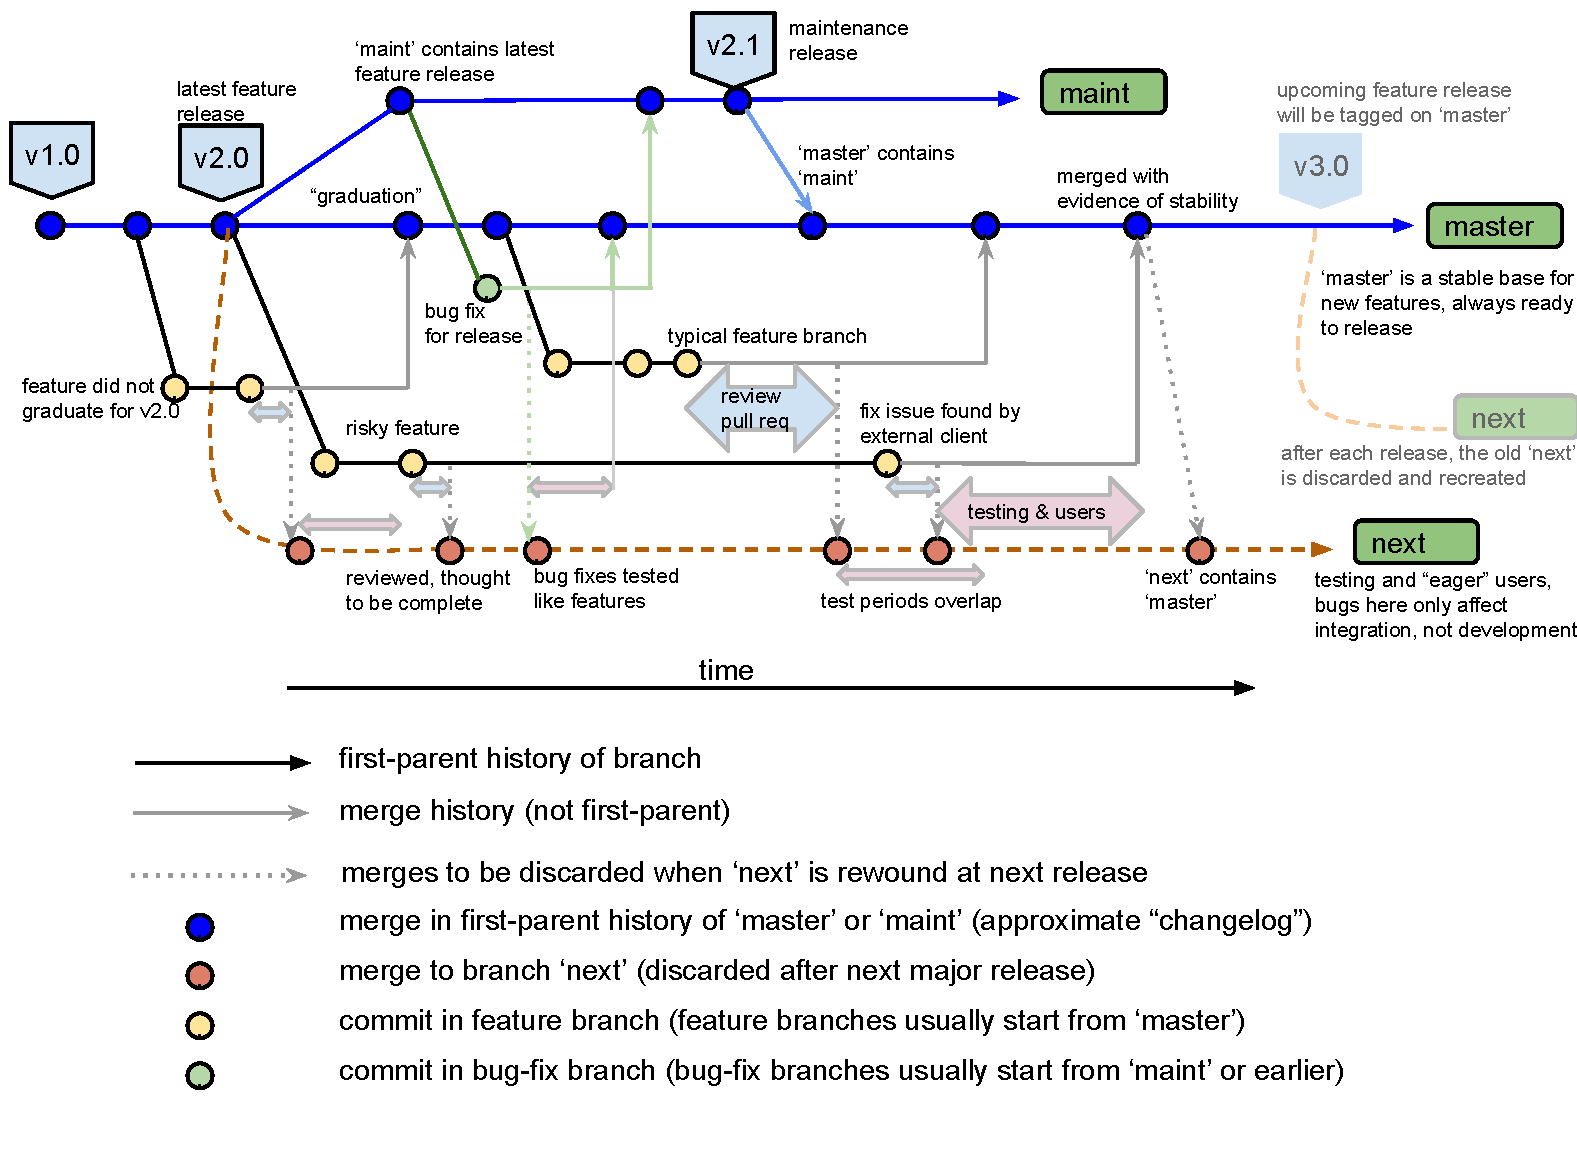
\includegraphics[width=\textwidth]{figures/Git/simplified-gitworkflows7.pdf}
\end{frame}



\section{Difficult and coupled problems}
\input{slides/FieldSplit.tex}
\input{slides/CoupledMultiphysics.tex}
\input{slides/Anisotropy.tex}
\begin{frame}{Algebraic Multigrid Tuning}
  \begin{itemize}
  \item Smoothed Aggregation (GAMG, ML)
    \begin{itemize}
    \item Graph/strength of connection -- MatSetBlockSize()
    \item Threshold (\code{-pc\_gamg\_threshold})
    \item Aggregate (MIS, HEM)
    \item Tentative prolongation -- MatSetNearNullSpace()
    \item Eigenvalue estimate
    \item Chebyshev smoothing bounds
    \end{itemize}
  \item BoomerAMG (Hypre)
    \begin{itemize}
    \item Strong threshold (\code{-pc\_hypre\_boomeramg\_strong\_threshold})
    \item Aggressive coarsening options
    \end{itemize}
  \end{itemize}
\end{frame}

\input{slides/SIPreconditioning.tex}

\section{PDE-constrained Optimization}
\begin{frame}{PDE-constrained optimization: Elliptic}
  \begin{gather*}
    \min_{u,y} \frac 1 2 \norm{Qy - d}^2 + \frac \alpha 2 \norm{L(u - u_{\text{ref}})}^2 \\
    \quad c(u,y) = 0
  \end{gather*}
  \begin{itemize}
  \item Design $u$, state $y$, data $d$
  \item $Q$ is an observation operator
  \item $L$ is cost functional for design
  \item $\alpha$ is tradeoff between cost of design and fitting data
  \item Equivalent to Bayesian MAP with uncorrelated standard Gaussian observation error and design prior
  \item Provide objective functional, gradient, (optionally) Hessian
  \item Constraint $c(u,y)$, Jacobian of constraint $\partial c/\partial u$ and $\partial c/\partial y$
  \item {\small \code{src/tao/pde\_constrained/examples/tutorials/elliptic.c}}
  \item Similar examples for parabolic and hyperbolic
  \end{itemize}
\end{frame}


\section{Recent developments in PETSc}
\subsection{Improved multiphysics support}
\begin{frame}{Multiphysics problems}
  \begin{block}{Examples}
    \begin{itemize}
    \item Saddle-point problems (\eg incompressibility, contact)
    \item Stiff waves (\eg low-Mach combustion)
    \item Mixed type (\eg radiation hydrodynamics, ALE free-surface flows)
    \item Multi-domain problems (\eg fluid-structure interaction)
    \item Full space PDE-constrained optimization
    \end{itemize}
  \end{block}
  \vspace{-0.5em}
  \begin{block}{Software/algorithmic considerations}
    \begin{itemize}
    \item Separate groups develop different ``physics'' components
    \item Do not know a priori which methods will have good algorithmic properties
    \item Achieving high throughput is more complicated
    \item Multiple time and/or spatial scales
      \begin{itemize}
      \item Splitting methods are delicate, often not in asymptotic regime
      \item Strongest nonlinearities usually non-stiff: explicit for TVD limiters/shocks
      \end{itemize}
    \end{itemize}
  \end{block}
\end{frame}

\input{slides/MonolithicOrSplit.tex}
\input{slides/PETSc/Coupling.tex}
\input{slides/PETSc/LocalSpaces.tex}
\input{slides/SNES/MultiphysicsAssemblyResiduals.tex}
\input{slides/SNES/MultiphysicsAssemblyJacobians.tex}
\input{slides/PETSc/MatGetLocalSubMatrix.tex}
\begin{frame}{SNES ex28}
  \begin{itemize}
  \item Example: {\kb src/snes/examples/tutorials/ex28.c}
  \item Solves a diffusion PDE for $u$
    $$-(k u_x)_x = 1$$
    on $(0,1)$, subject to $u(0) = 0, u(1) = 1$
  \item with implicitly defined coefficient $k$ solving
    $\exp(k-1) + k = 1/\Big(1/(1+u) + 1/(1+u_x^2)\Big)$
  \end{itemize}
\end{frame}
\subsection{Variational inequalities}
\input{slides/PETSc/SNESVI.tex}

\begin{frame}{References}
  \begin{itemize}
  \item Knoll and Keyes, \emph{Jacobian-free Newton-Krylov methods: a survey of approaches and applications}, JCP, 2004.
  \item Elman et. al., \emph{A Taxonomy and Comparison of Parallel Block Multi-Level Preconditioners for the Incompressible Navier-Stokes Equations}, JCP, 2008.
  \item Wan, Chan, and Smith, \emph{An Energy-minimizing Interpolation for Robust Multigrid Methods}, SIAM J. Sci. Comp, 2000.
  \item Gropp, Kaushik, Keyes, Smith, \emph{Performance Modeling and Tuning of an Unstructured Mesh CFD Application}, Supercomputing, 2000.
  \item Gropp, \emph{Exploiting Existing Software in Libraries: Successes, Failures, and Reasons Why}, OO methods for interoperable scientific and engineering computing, 1999.
  \item ICiS Multiphysics workshop report:  IJHPCA 27(1), Feb 2013, http://dx.doi.org/10.1177/1094342012468181
  \end{itemize}
\end{frame}

\end{document}
